\input{/Users/daniel/github/config/preamble.sty}
\input{/Users/daniel/github/config/ops.sty}

\begin{document}
{\LARGE Summary of algebraic topology II}

\tableofcontents

\section{Basic notions}\label{sec:Basic notions}
\subsection{Defintions}
\paragraph{Two introductory paragraphs from Tom Diek}
\begin{itemize}
	\item Let $X$ and $Y$ be topological spaces and $f,g:X\to Y$ continuous maps. An \textbf{\textit{homotopy}} from $f$ to $g$ is a continuous map
		\[H:X\times[0,1]\to Y,\qquad(x,t)\mapsto H(x,t)=H_t(x)\]
		such that $f(x)=H(x,0)$ and $g(x)=H(x,1)$ for all $x\in X$. We denote this situation by $f\simeq g$. The homotopy relation $\simeq$ is an equivalence relation on the set of continuous maps $X\to Y$. A homotopy of maps $H_t:X\to Y$ is called \textbf{\textit{relative to $A\subset X$}} if $H_t|_A$ is constant.
		
		\item Topological spaces and homotopy classes of maps form a quotient category of $\Top$, the \textbf{\textit{homotopy category $\hTop$}}, where comoposition of homotopy classes is induced by composition of representing maps. If $f:X\to Y$ represents an isomorphism in $\hTop$, then $f$ is called a \textbf{\textit{homotopy equivalence}} or \textbf{\textit{$\operatorname{h}$-equivalence}}. In explicit termins this means $f:X\to Y$ is a homotopy equivalence if there exists $g:Y\to X$, a \textbf{\textit{homotopy inverse of $f$}}, such that $gf$ and $fg$ are both homotopic to the identity. Spaces $X$ and $Y$ are called \textbf{\textit{homotopy equivalent}} or of the same \textbf{\textit{homotopy type}} if there exists a homotopy equivalence $X\to Y$. A space is \textbf{\textit{contractible}} if it is homotopy equivalent to a point. A map $f:X\to Y$ is \textbf{\textit{null homotopic}} if it is homotopic to a constant map.
\end{itemize}

\subsubsection{\texorpdfstring{$n$}{n}-th homotopy group of a pointed space}

\begin{defn}[Homotopy groups]
	Let $(X,x_0)$ be a pointed topological space and $s_0\in S^n$. The elements of the \textbf{\textit{$n$-th homotopy group}} are homotopy classes of maps $(S^n,s_0)\to (X,x_0)$. Equivalently, they are homotopy classes of maps $(I^n,\partial I^n)\to (X,x_0)$. (Homotopies are required to preserve the base points, $s_0\mapsto x_0$ or $\partial I^n\mapsto x_0$.)
		
	Also,
	\[\pi_n(X,*)=[(I^n,\partial I^n),(X,\{*\})]\cong[I^n/\partial I^n,X]^0\]
	where $[X,Y]$ denotes the set of homotopy classes $[f]$ of maps $[f]:X\to Y$.
\end{defn}

\subsubsection{\texorpdfstring{$n$}{n}-th relative homotopy group of a pointed pair of spaces}
Let $A$ be a subspace of $X$ and $x_0\in A$. The elements of the \textbf{\textit{relative homotopy group $\pi_n(X,A,x_0)$}} are homotopy classes of maps $(I^n,\partial I^n,J^{n-1})\to (X,A,x_0)$ where $J^{n-1}$ is the union of all but one face of $I^n$. That is,
		\[\pi_{n+1}(X,A,*)=[(I^{n+1},\partial I^{n+1},J^n),(X,A,x_0)].\]
		
		The elements of such a group are homotopy classes of based maps $D^n\to X$ which carry the boundary $S^{n-1}$ into $A$. Two maps $f,g$ are called \textbf{\textit{homotopic relative to $A$}} if they are homotopic by a basepoint-preserving homotopy $F:D_n\times[0,1]\to X$ such that, for each $p$ in $S^{n-1}$ and $t$ in $[0,1]$, the element $F(p,t)$ is in $A$. Ordinary homotopy groups are recovered for the case in which $A=\{x_0\}$.
\begin{remark}
	This construction is motivated by looking for the kernel of the induced map $i_*:\pi_n(A,x_0)\to\pi_n(X,x_0)$ by the inclusion. This map is in general not injective, and the kernel consists of ?
\end{remark}

\subsection{Commutativty of higher homotopy groups}
\begin{prop}
	$\pi_n(X,x_0)$ is an abelian group for all $n\in\N$.
\end{prop}

\subsection{Action of fundamental grupoid \texorpdfstring{$\Pi_1(X)$}{Π₁(X)} of \texorpdfstring{$X$}{X} on \texorpdfstring{$\pi_{n}(X)$}{π₁(X)}}
\begin{itemize}
	\item A \textit{\textbf{groupoid}} is a small category in which every morphism is an isomorphis.
	\item The \textit{\textbf{fundamental groupoid}} $\Pi_{1}(X)$ is the category whose objects are the points of  $X$ and morphisms are homotopy classes of paths joining two points.Composition is defined doubling the speed.
\end{itemize}

The fundamental groupoid acts on homotopy group functorially.

\subsection{Action of fundamental grupoid \texorpdfstring{$\Pi_1(X)$}{Π₁(X)} of \texorpdfstring{$A$}{A} on \texorpdfstring{$\pi_{n}(X,A)$}{π₁(X,A)}}

\subsection{Homotopy groups of a product of spaces are products of homotopy groups of factors}

\subsection{Higher homotopy groups of a covering space are the same as those of a base space}

\subsection{Long exact sequence of homotopy groups associated to a pair}

For any pair $(X,A,x)$ we have a long exact sequence
\[\begin{tikzcd}[column sep=small]
	\pi_n(A,x_0)\arrow[r,"i_*"]&\pi_{n}(X,x_0)\arrow[r,"j_*"]&\pi_{n-1}(X,A,x_0)\arrow[r,"\partial"]&\pi_{n-1}(A,x_0)\arrow[r]&\cdots\arrow[r]&\pi_0(X,x_0)
\end{tikzcd}\]
where $i$ and $j$ are the inclusions $(A,x_0)\hookrightarrow(X,x_0)$ and $(X,x_0,x_0)\hookrightarrow(X,A,x_0)$. The map $\partial$ comes from restricting maps $(I^n,\partial I^n,J^{n-1})\to (X,A,x_0)$ to $I^{n-1}$, or by restricting maps $(D^n,S^{n-1},s_0)\to (X,A,x_0)$. The map, called the \textbf{\textit{boundary map}}, is a homomorphism when $n>1$.

\subsection{\texorpdfstring{$n$}{n}-connected space}

A space $X$ with basepoint $x_0$ is called \textbf{\textit{$n$-connected}} if $\pi_i(X,x_0)=0$ for $i\leq n$. Thus 0-connected means path-connected and 1 connected means simply-connected.

\subsection{\texorpdfstring{$n$}{n}-connected pair}

A pair $(X,A)$ is \textbf{\textit{$n$-connected}} if $\pi(X,A,x_0)=0$ for $i\leq n$.

\subsection{$n$-equivalnce of spaces}

A map $f:X\to Y$ is an \textit{\textbf{ $n$-equivalence}} if the induced map on homotopy groups $f_{*}:\pi_{i}(X)\to \pi_{i}(Y)$ is an isomorphism for $i<n$ and a surjection for $i=n$.

\begin{remark}\leavevmode
	\begin{itemize}
		\item $(X,A)$ is $n$-connected if and only if $A\hookrightarrow X$ is an $n$-equivalence.
		\item $f:X\to Y$ is an $n$-equivalence if and only if when we replace $f$ by a cofibration $X\to M_{f}$, $(M_{f},X)$ is $n$-connected.
	\end{itemize}
\end{remark}

\section{Cartesian closed structure}

\subsection{Definitions}

\subsubsection{Cartesian closed category}

[Taken from homework 1]
	In the category of sets there is a bijection $\Hom(X\times Y, Z)\cong \Hom(X, \Hom(Y, Z))$ that depends naturally on $X$, $Y$ and $Z$. The notions related to this bijection are “Cartesian closed category”, “currying” and “internal Hom”.
\begin{defn}
	A category $\Cc$ is \textbf{\textit{Cartesian closed}} if:
	\begin{enumerate}
		\item $\Cc$ has all finite products (Caveat: some require that $\Cc$ has all finite limits)
		\item For any object $Y$ the functor $- \times Y$ has a right adjoint, which we will denote by $\Map(Y,-)$ or by $-^Y$ .
	\end{enumerate}
\end{defn}
\begin{remark}
	By section 3 \href{https://ncatlab.org/nlab/show/internal+hom }{here}, the second property above implies that we get a functor $\Map(-,-) : \Cc^{\op} \times \Cc \to \Cc$, and moreover we get natural isomorphisms $\Hom(X, \Map(Y, Z)) \cong \Hom(X \times Y, Z)$ and $\Map(X, \Map(Y, Z))\cong \Map(X \times Y, Z)$.
\end{remark}

\subsubsection{Compactly generated space}

\begin{claim}[What I picked up from the lecture]
		If $X$ is compactly generated, then $X$ is weakly Hausdorff if the diagonal subset $\Delta_X\subset X\times X$ is {\color{orange}$k$-closed}.
\end{claim}
	 Now some other notes from the lectures:
	
	In $\CGWH$, $\Hom(X,Y)$ is a space with the compact-open topology. This is a compactly generated space, $\mathbf{k}(\Hom(X,Y))$.
\begin{remark}
	(Also see \href{https://en.wikipedia.org/wiki/Currying#Function_spaces}{wiki on currying})
	\begin{align*}
		\Map(X,Y):=\text{ the space of maps }X\to Y.\\
		\Map(X\times Y,Z)\cong\Map(X,\Map(Y,Z))\\
		\Hom(X\times Y,Z)\cong \Hom(X,\Map(Y,Z))
	\end{align*}
	In the last line, product is product in $\CGWH$, not in $\Top$.
	The functor $-\times Y$ is left adjoint to $\Map(Y,-)$.

\begin{quotation}
	We don't care so much about $\Top$. We care much more about $\CGWH$, the full subcategory of $\Top$ on \textbf{\textit{compactly generated wakly Hausdorff}} spaces.
\end{quotation}
\begin{defn}[{\color{magenta}Is this right?}]
	$X$ is \textbf{\textit{compactly generated}} if, for any subset $C\subset X$, and for all continuous maps $f:K\to X$ from compact Housdorff spaces, \[\text{if } f^{-1}(C) \text{is closed in }K\text{, then } C\text{ is closed}.\]
\end{defn}
\begin{claim}
	If $X$ is compactly generated, then $X$ is weakly Hausdorff if the diagonal subset $\Delta_X\subset X\times X$ is {\color{orange}$k$-closed}.
\end{claim}

\paragraph{Explanation from the book of May} The ordinary category of spaces allows pathology that obstructs a clean development of the foundations. The homotopy and homology groups of spaces are supported on compact subspaces, and it turns out that if one assumes a separation property that is a little weaker than the Hausdorff property, then one can refine the point-set topology of spaces to eliminate such pathology without changing these invariants.
	
	One major source of point-set level pathology can be passage to quotient spaces. Use of compactly generated topologies alleviates this.
	\begin{prop}
		If $X$ is compactly generated and $\pi:X\to Y$ is a quotient map, then $Y$ is compactly generated if and only if $(\pi\times \pi)^{-1}(\Delta Y)$ is closed in $X\times X$
	\end{prop}
	The interpretation is that a quotient space of a compactly generated space by a “closed equivalence relation” is compactly generated.

\subsubsection{Weakly Housdorff space}

\subsection{Cartesian closedness of the category $CGWH$}
See "Compactly generated spaces" by Charles Rezk.

\subsection{Wedge}

\subsection{Smash product of spaces, its associativity in \texorpdfstring{$\operatorname{CGWH}$}{CGWH}}

The appropriate analogue of the Cartesian product in the category of based spaces is the \textbf{\textit{smash product}} $X\wedge Y$ defined by
	\[X\wedge Y=X\times Y/X\vee Y.\]
	Here $X\vee Y$ is viewed as the subspace of $X\times Y$ consisting of those pairs $(x,y)$ such that either $x$ is the basepoint of $X$ or $y$ is the basepoint of $Y$.
\end{defn}
\begin{example}[Basic example]
	The smash product of two circles is a sphere, as may be seen by collapsing the generating circles on a revolution torus (see \href{https://en.wikipedia.org/wiki/Smash_product#/media/File:Visualization_of_the_smash_product_of_two_circles.gif}{Wikipedia}).
\end{example}

\subsection{Reduced and unreduced suspension}
We also have the \textbf{\textit{suspension of pointed spaces}}, which is like usual suspension but also collapsing the distinguished point, which has become an interval:
\[\Sigma X=(I\times X)/(t,x)\sim (0,y)\sim (1,y)\;\forall y\in X.\]

\subsection{Path and loop spaces of a pointed space}
[This is defined in Hatcher close to the homotopy fiber construction--- it's related to Blakers-Massey, Freudenthal theorem.]

\begin{defn}[Path fibration]
	An important case of the homotopy fiber construction is when the given function $f$ is the inclusion of the basepoint $b_0$ into $B$. Then $E_{f}$ is the space $PB$ of paths in $B$ starting at $b_{0}$,  and $p:PB\to B$ sends each path to its endpoint. The fiber $p^{-1}(b_{0})$ is the loopspace $\Omega B$ consisting of all loops in  $B$ based at $b_{0}$. Since $PB$ is contractible by progressively truncating paths, the long exact sequence of homotopy groups for the path fibration yields (another proof that)
	\[\pi_{n}(X,x_{0})\cong \pi_{n-1}(\Omega X,x_{0})\qquad \forall n.\]
\end{defn}

\subsection{For pointed spaces: smash with any \texorpdfstring{$Y$}{Y}		 is adjoint to  \texorpdfstring{$\operatorname{Map}(Y,-)$}{Map(Y,-)}}
[From \href{https://en.wikipedia.org/wiki/Smash_product#}{Wikipedia}]
Adjoint functors make the analogy between the tensor product and the smash product more precise. In the category of $R$-modules over a commutative ring $R$, the tensor functor $(-\otimes_{A} A)$ is left adjoint to the internal Hom functor $\Hom(A,-)$, so that
\[\operatorname{Hom}(X\otimes A,Y)\cong \operatorname{Hom}(X,\operatorname{Hom}(A,Y)).\]
In the category of pointed spaces, the smash product plays the role the tensor product in this formula: if $A$, $X$ are compact Hausdorff then we have an adjunction
\[\operatorname{Maps}_{*}(X\wedge A,Y)\cong \operatorname{Maps}_{*}(X,\operatorname{Maps}_{*}(A,Y))\]
where $\operatorname{Maps}_{*}$ denotes continuous maps that send basepoint to basepoint, and $\operatorname{Maps}_{*}(A,Y)$ carries the compact-open topology.

\subsection{Adjointness of \texorpdfstring{$\Sigma$}{Σ} and \texorpdfstring{$\Omega$}{Ω}}
In particular, taking $A$ to be the unit circle $S^{1}$, we see that the reduced suspension functor $\Sigma$ is left adjoint to the loop space functor $\Omega$:
\[\operatorname{Maps}_{*}(\Sigma X,Y)\cong \operatorname{Maps}_{*}(X,\Omega Y).\]

[From lectures:] Then we have
\[\Hom_{\CGWH_*}(\Sigma X,\Sigma X)\cong\Hom_{\CGWH_*}(X,\Omega\Sigma X)\]
where $\Sigma X=S\wedge X$ and $\Omega\Sigma X=\Map(S^1,\Sigma X)$. That is, $S^1\wedge-$ is adjoint to $\Map(S^1,-)$.

\subsection{CW-complex, relative CW-complex}
\subsection{Topology on product of CW-complexes is the same as product topology in $CGWH$}

\section{Homotopy theory  of spaces (A)}
\subsection{Definitions}
\subsubsection{Weak factorization system}

Here we follow \href{https://arxiv.org/pdf/1904.0088}{Rihel, Homotopical categories: from model categories to $(\infty,1)$-categories}

\begin{defn}
	A \textbf{\textit{weak factorization system $(\Lc,\Rc)$}} on a category $\Mc$ is comprised of two clases of morphisms $\Lc$ and $\Rc$ so that
	\begin{enumerate}
		\item Every morphism in $\Mc$ may be factored as a morphism in $\Lc$ followed by a morphism in $\Rc$:
		\[\begin{tikzcd}
			\bullet\arrow[rr,"f"]\arrow[rd,"\Lc\ni\ell",swap]&&\bullet\\
			&\bullet\arrow[ru,"r\in\Rc",swap]
		\end{tikzcd}\]
		\item The maps in $\Lc$ have the \textbf{\textit{left lifting property}} with respect to each map in $\Rc$ and equivalently the maps in $\Rc$ have the \textbf{\textit{right lifting property}} with respect to each map in $\Lc$, that is, any commutative square
		\[\begin{tikzcd}
			\bullet\arrow[d,"\Lc\ni\ell",swap]\arrow[r]&\bullet\arrow[d,"r\in\Rc"]\\
			\bullet\arrow[ur,dashed]\arrow[r]&\bullet
		\end{tikzcd}\]
		admits a diagonal filler as indicated making both triangles commute. When this lift is unique, we say the factorization system is \textbf{\textit{orthogonal}}.
		\item The classes $\Lc$ and $\Rc$ are each closed under retracts in the arrow category: given a commutative diagram
		\[\begin{tikzcd}
			\bullet\arrow[r]\arrow[d,"t",swap]\arrow[rr,bend left,no head,shift left=.3]\arrow[rr,bend left,no head,shift right=.3]&\bullet\arrow[r]\arrow[d,"s"]&\bullet\arrow[d,"t"]\\
			\bullet\arrow[r]\arrow[rr,bend right,no head, shift right=.3]\arrow[rr,bend right,no head, shift left=.3]&\bullet\arrow[r]&\bullet
		\end{tikzcd}\]
		if $s$ is in that class then so is its retract $t$.
	\end{enumerate}
\end{defn}

\begin{exercise}[3.1.8, Rihel]
Verify that the class of morphisms $\Lc$ characterized by the left lifting property against a fixed class of morphisms $\Rc$ is closed under coproducts, closed under retracts, and contains the isomorphisms.
\end{exercise}

\subsubsection{Model category structure on a category}

\begin{defn}[Lecture]
	A \textbf{\textit{model structure}} on a category $\Ac$ is a choice of subcategories $\Wc,\Cc,\Fc$ called \textbf{\textit{weak-equivalences}}, \textbf{\textit{cofibrations}} and \textbf{\textit{fibrations}} with the following properties:
	\begin{enumerate}
		\item[0.] All (finite) small limits an colimits.
		\item \textbf{(2 of 3)} Given $\bullet\overset{f}{\to}\bullet\overset{g}{\to}\bullet$, if either 2 out of 3 among $f,g,f\circ g$ are in $\Wc$ then all of them are.
		\item $(\Cc\cap\Wc,\Fc)$ and $(\Cc,\Fc\cap\Wc)$ are both weak factorization systems.
		$(\Bc,\Dc)$ is a weak factorization system. That is,
		\begin{enumerate}
			\item Any morphism in $\Ac$ can be factored as a morphism in $\Bc$ followed by a morphism in $\Dc$.
			\item Lifts:
			\[\begin{tikzcd}[scale cd=1.2]
				\bullet\arrow["f",d,swap]\arrow[r]&\bullet\arrow[d,"g"]\\
				\bullet\arrow[ur,dashed,"\exists"]\arrow[r]&\bullet
			\end{tikzcd}\]
			\item[(c')] Notice that the axiom of retracts is not necessary. $r'\in\Rc\iff$ it satisfies (b) for all $\ell\in\Lc$.
 		\end{enumerate}
	\end{enumerate}
\end{defn}

\begin{defn}\leavevmode
	\begin{itemize}
		\item $X$ is \textbf{\textit{fibrant}} if $X\twoheadrightarrow\pt$.
		\item $X$ is \textbf{\textit{cofibrant}} if \begin{tikzcd}
			X\arrow[r,tail,two heads]&X
		\end{tikzcd}
		\item $X$ is \textbf{\textit{bifibrant}} if \begin{tikzcd}
			0\arrow[r,tail]&X\arrow[r,two heads]&\pt
		\end{tikzcd}
	\end{itemize}
\end{defn}

\subsection{Str\o m and Quillen model structures}

\begin{example}[Two interesting model category structures on $\CGWH$]\leavevmode
\begin{enumerate}
	\item \textbf{\textit{Hurewicz-Str\o m model structure}}.
	\begin{itemize}
		\item Cofibrations = Huerwicz cofibrations.
		\item Fibrations = Hurewicz fibrations.
		\item Weak equivalences = homotopy equivalences.
	\end{itemize}
	\item \textbf{\textit{Quillen model structure}}. Defined on $\Top$.
	\begin{itemize}
		\item Cofibrations = "retracts of relative cell complexes".
		\item Fibrations = Serre fibrations.
		\item Weak equivalences = weak homotopy equivalences.
	\end{itemize}
\end{enumerate}
\end{example}

\subsection{Hurewicz fibrations and cofibrations}

\subsubsection{Fibrations}

\begin{defn}[Hatcher]
	 A map $p:E\to B$ is said to have the \textbf{\textit{homotopy lifting property}} with respect to a space $X$ if, given a homotopy $g_t:X\to B$ and a map $\tilde{g}_0:X\to E$ lifting $g_0$, so $p\tilde{g}_0=g_0$, then there exists a homotopy $\tilde{g}_t:X\to E$ lifting $g_t$.
	
	The \textbf{\textit{lift extension property for a pair $(Z,A)$}} asserts that every map $X\to B$ has a lift $Z\to E$ extending a given lift defined on the subspace $A\subset Z$. The case $(Z,A)=(X\times I,X\times\{0\})$ is the homotopy lifting property.
	
	A \textbf{\textit{fibration}} is a map $p:E\to B$ having the homotopy property with respect to all spaces $X$.
\end{defn}

\begin{defn}[\href{https://ncatlab.org/nlab/show/lift}{nLab}]
	A morphism $i$ has the \textbf{\textit{left lifting property with respect to a morphism $p$}} and $p$ has the \textbf{\textit{right lifting property with respect to $i$}} if for each morphisms $f$ and $g$, if the outer square in the following diagram commutes, there exists $\phi$ (I think not necessarily unique) completing the diagram:
	\[\begin{tikzcd}[row sep=large]
		A\arrow[r,"f"]\arrow[d,"i",swap]&X\arrow[d,"p"]\\
		B\arrow[r,"g",swap]\arrow[ur,dashed,"\phi"]&Y
	\end{tikzcd}\]
\end{defn}

\begin{defn}[\href{https://ncatlab.org/nlab/show/homotopy+lifting+property}{nLab}] Let $C$ be a category with products and with interval object $I$. A morphism $E\to B$ has the \textbf{\textit{homotopy lifting property}} if it has the right lifting property with respect to all morphisms of the form $(\id,0):Y\to Y\times I$.
	
	This means that for all commuting squares
	\[\begin{tikzcd}
		Y\arrow[r,"f"]\arrow[d]&E\arrow[d,"p"]\\
		Y\times I\arrow[r,swap,"F"]\arrow[ur,dashed,"\sigma"]&B
	\end{tikzcd}\]
	there exists a morphism $\sigma:Y\times I\to E$ such that both triangles in the former diagram commute.
	
	A \textbf{\textit{fibration}} (also called \textbf{\textit{Hurewicz fibration}}) is a mapping $p:E\to B$ satisfying the homotopy lifting property for all spaces $X$.
\end{defn}

\subsubsection{Cofibrations}

\begin{defn}[Hatcher]
	If in the definition of a fibration as a map satisfying the homotopy lifting property we reverse the direction of the arrows, we obtain the dual notion of a \textit{\textbf{cofibration}}. This is a map $i:A\to B$ {\color{persimmon}(which is $E\to B$ backwards)} satisfying the following property: {\color{persimmon}(we used to have an homotopy from some space $X$ into the base, now we have:)} given an homotopy $g_{t}:A\to X$ and {\color{persimmon}(a lift)}  $\tilde{g}:B\to X$ such that $\tilde{g}_{0}i=g_{0}$, there exists a homotopy $\tilde{g}_{0}:B\to X$ such that $\tilde{g}_{t}i=g_{t}$.

	In the special case that $i$ is the inclusion of a subspace, this is the homotopy extension property, and the next proposition says that this is indeed the general case. So a cofibration is an inclusion satisfying the homotopy extension property.
\end{defn}

\begin{prop}[4H.1]
	If $i:A\to B$ is a cofibration, then $i$ is injective, and in fact a homeomorphism onto its image.
\end{prop}

\begin{remark}[From Hatcher p. 461]
	The duality between subobjects and quotient objects is clear for abelian groups, where subobjects are kernels and quotient objects cokernels. The strict topological analog of a kernel is a fiber of a fibration. Dually, the topological analog of a cokernel is the \textit{\textbf{cofiber}} $B/A$ of a cofibration $A\hookrightarrow B$. If we make an arbitrary map  $f:A\to B$ into a cofibration $A\hookrightarrow M_{f}$, the cofiber is the mapping cone $C_{f}=M_{f}/(A\times {0}$.
\end{remark}

\begin{defn}[\href{https://en.wikipedia.org/wiki/Homotopy_extension_property}{wiki}]
	Let $X$ be a topological space and let $A\subset X$. We say that the pair $(X,A)$ has the \textbf{\textit{homotopy extension property}} if, given a homotopy $f_\bullet:A\to Y^I$ and a map $\tilde{f}_0:X\to Y$ such that
		\[\tilde{f}_0\circ\iota=f_0\]\
		{\color{cyan}(so $\tilde{f}$ is the lift of $f_0:A\to Y$)} then there exists an \textbf{\textit{extension}} of $f_\bullet$ to a homotopy $\tilde{f}_\bullet:X\to Y^I$ such that $\tilde{f}_\bullet\circ\iota=f_\bullet$.
		
		That is,
		\[\begin{tikzcd}
			A\arrow[r,"f_\bullet"]\arrow[d,swap,"\iota"]&Y^I\arrow[d,"\pi_0"]\\
			X\arrow[ur,dashed,"\tilde{f}_\bullet"]\arrow[r,swap,"\tilde{f}_0"]&Y
		\end{tikzcd}\]
		{\color{persimmon}So there's some \href{https://en.wikipedia.org/wiki/Currying#Function_spaces}{currying} to make usual homotopies $f_\bullet:A\times I\to Y$ look like $f_\bullet:A\to Y^I$. As said in our lectures: ``a homotopy $X\times I\to Y$ is the same as a map $X\to \Map(I,Y)$".}

	A map $\iota:A\to X$ is a \textit{\textbf{cofibration}} if it has the homotopy extension property with respect to all topological spaces  $Y$.
\end{defn}

\subsubsection{Mapping cylinder}

\begin{defn}[\href{https://ncatlab.org/nlab/show/mapping+cylinder}{nLab}]
	Given a continuous map $f:X\to Y$ of topological spaces, one can define its \textbf{\textit{mapping cylinder}} as a pushout
	\[\begin{tikzcd}
		X\arrow[r,"f"]\arrow[d]&Y\arrow[d]\\
		X\times I\arrow[r,swap,"(\sigma_0)_*(f)"]&\Cyl(f)
	\end{tikzcd}\]
	in $\Top$, where $I=[0,1]$ and $\sigma:X\to X\times I$ is given by $x\mapsto(x,0)$.
	
	Set theoretically, the mapping cyllinder is usually represented as que quotient space
	\[\left(X\times I\coprod Y\right)\Big/\sim\]
	where $\sim$ is the smallest equivalence relation identifying $(x,0)\sim f(x)$ for all $x\in X$.
\end{defn}

\begin{defn}[\href{https://en.wikipedia.org/wiki/Mapping_cylinder}{wiki}]
	The \textbf{\textit{mapping cylinder}} of a function $f$ between topological spaces $X$ and $Y$ is the quotient
	\[M_f=(([0,1]\times X)\amalg Y)\big/\sim\]
	where $\amalg$ denotes disjoint union, and $\sim$ is the equivalence relation generated by
	\[(0,x)\sim f(x)\text{ for each }x\in X.\]
	{\color{persiangreen}That is, the mapping cylinder $M_f$ is obtained by gluing one end of $X\times[0,1]$ to $Y$ via the map $f$.} Notice that the ``top" of the cylinder $\{1\}\times X$ is homeomorphic to $X$, while the ``bottom" is the space $f(X)\subset Y$.
	
{\color{persiangreen}Looks the mapping cylinder is just deforming $X$ to $Y$ putting $X$ inside $Y$ via $f$…}
\end{defn}

\begin{defn}[From homework]
	Let $f:X\to Y$ be a map. Let $M_f=X\times[0,1]\cup_fY$ be the \textbf{\textit{mapping cylinder of $f$}}, i.e. the pushout of $X\overset{\cong}{\to}X\times\{0\}\hookrightarrow X\times[0,1]$ and of $f:X\times Y$.
\end{defn}

\subsection{Serre fibrations}

\begin{defn}[Hatcher, p. 376]
		The map $p:E\to B$ is said to have the \textbf{\textit{homotopy lifting property for a pair}} $(X,A)$ if each homotopy $f_t:X\to B$ lifts to a homotopy $\tilde{g}_t:X\to E$ starting with a given lift $\tilde{g}_0$ and extending a given lift $\tilde{g}_t:A\to E$. In other words, the homotopy lifting property for $(X,A)$ is the lift extension property for $(X\times I,X\times\{0\}\cup A\times I)$.
	
	The important observation here is that homotopy lifting property for disks is equivalent to the homotopy lifting property for all CW pairs $(X,A)$. A map $p:E\to B$ satisfying the homotopy lifting property for disks is sometimes called a \textbf{\textit{Serre fibration}}.
\end{defn}

\subsection{Fiber bundles}

Here I include some more notes of the discussion following Serre fibrations on Hatcher.

	A \textbf{\textit{fiber bundle}} structure on a space $E$, with fiber $F$, consists of a projection map $p:E\to B$ such that each point $B$ has a neighbourhood $U$ for which there is a homeomorphism $h:p^{-1}(U)\to U\times F$ making the following diagram commute
	\[\begin{tikzcd}
		p^{-1}(U)\arrow[rr,"h"]\arrow[dr,"p"]&&U\times F\arrow[dl]\\
		&U
	\end{tikzcd}\]
\end{itemize}

\begin{example}
	Projective spaces yield interesting fiber bundles. In the real case we have the familiar covering spaces $S^n\to\R P^n$ with fiber $S^0$. Over the complex numbers the analog of this is a fiber bundle $S^1\to S^{2n+1}\to\C P^n$. Here $S^{2n+1}$ is the unit sphere in $\C^{n+1}$ and $\C P^n$ is viewed as the quotient space of $S^{2n+1}$ under the equivalence relation $(z_0,\ldots,z_n)\sim\lambda(z_0,\ldots,z_n)$ {\color{orange}for $\lambda\in S^1$}. The projection $p:S^{2n+1}\to\C P^n$ sends $(z_0,\ldots,z_n)$ to its equivalence class $[z_0,\ldots,z_n]$.
	
	To see that the local triviality condition for fibre bundles is satisfied, …
	
	The constructino of the bundle $S^1\to S^{2n+1}\to\C P^n$ also works when $n=\infty$, so there is a fiber bundle $S^1\to S^\infty\to \C P^\infty$.
	
	The case $n=1$ is particularly interesting since $\C P^1=S^2$ and bundle becomes $S^1\to S^3\to S^2$ with fiber, total space, and base all speres. This is known as the \textbf{\textit{Hopf bundle}}. The projection $S^3\to S^2$ can be taken to be $(z_0,z_1)\mapsto z_0/z_1\in\C\cup\{\infty\}=S^2$. {\color{persiangreen}(That is, seeing $S^2$ as the one-point compactification of $\C$.)}
	
	In polar coordinates we may see $S^3$ as the union of several tori. Stereorgraphic projection yields the following figure:
	\begin{figure}[H]
		\centering
		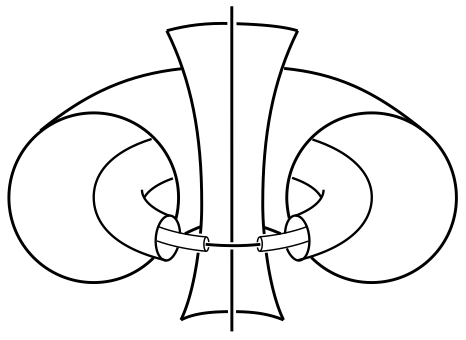
\includegraphics[width=0.5\linewidth]{hopf-bundle}
		\label{fig:hopf-bundle}
	\end{figure}
	The limiting cases $T_0$ and $T_\infty$ correspond to the unit circle in the $xy$-plane and the $z$-axis under the stereographic projection.	Each torus $T_\rho$ is aunion of circle fibers. These fiber circles have slope 1 on the torus, winding around once longitudinally and once meridionally. As $\rho$ goes to $0$ or $\infty$ the fiber circles approach the circles $T_0$ and $T_\infty$, which are also fibers. The figure below shows four tori decomposed into fibers:
	\begin{figure}[H]
		\centering
		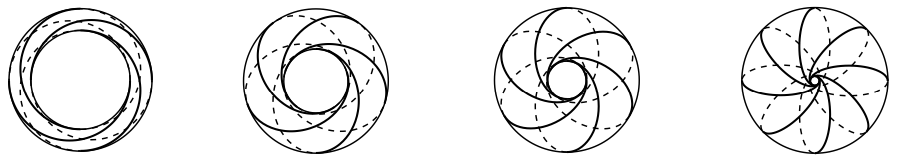
\includegraphics[width=0.9\linewidth]{hopf-bundle2}
		\label{fig:hopf-bundle2}
	\end{figure}
	
	Replacing the field $\C$ by the quaternions $\H$, the same constructions yield fiber bundles $S^3\to S^{4n+3}\to\H P^{n}$ over quaternionic projective spaces $\H P^n$. Here the fiber $S^3$ is the unit quaternions, and $S^{4n+3}$ is the unit sphere in $\H^{n+1}$. Taking $n=1$ gives a second Hopf bundle $S^3\to S^7\to S^4=\H P^1$.
	
	Another Hopf bundle $S^7\to S^{15}\to S^8$…
\end{example}

\subsection{Homotopy equivalences and weak homotopy equivalences}

\begin{defn}[Weak homotopy equivalence]
	Any map $f:X\to Y$ that induces isomorphisms on all homotopy groups ( $\forall n\geq 0$ and all choices of basepoint in $X$).
\end{defn}

\subsection{Any Hurewicz fibration is Serre fibration}
\subsection{Any relative CW-complex is a cofibration in Quillen model structure}
\subsection{Any map can be replaced by…} 
\subsubsection{an homotopy equivalence followed by Hurewicz fibration}
\subsubsection{a Hurewicz cofibration followed by homotopy equivalence}
\subsubsection{a Quillen cofibration followed by weak equivalence}
This one follows from CW-approximation theorem

\section{Homotopy theory  of spaces (B)}

\subsection{Blakers-Massey theorem}

As in Hatcher and in terms of homotopy pullbacks and pushouts. (Be careful if you refer to REsk's paper for the latter version, since in his paper the $n$ in definition of $n$-connectiviy is shifted by $1$.
\begin{thm}[Blakers-Massey. Hatcher 4.23, Tom Dieck 6.4.1]
	Let $X$ be a CW complex decomposed as the union of subcomplexes $A$ and $B$ with nonempty connected intersection $C=A\cap B$ {\color{magenta}(that is also a CW complex?)}. If $(A,C)$ is $m$-connected and $(B,C)$ is $n$-connected, $m,n\geq 0$, then the map
	\[\pi_{i}(A,C)\to \pi_{i}(X,B)\]
is an isomorphism for $i<m+n$ and a surjection for $i=m+n$.
\end{thm}

\begin{prop}[Quotient theorem. Hatcher, 4.28and Tom Dieck 6.10.2]
	If a CW pair $(X,A)$ is $r$-connected and $A$ is $r,s \geq 0$, then the map $\pi_{i}(X,A)\to \pi_{n}(X/A)$ induced by the quotient map $X\to X/A$ is an isomorphism for $i\leq r+s$ and a surjection for $i=r+s+1$.
\end{prop}
\begin{proof}
	Using cones.
\end{proof}

\subsection{Freudethal suspension theorem}

\begin{coro}[Freudenthal suspension theorem, Hatcher 4.24]
	The suspension map $\pi_{i}(S^{n})\to \pi_{i+1}(S^{n+1})$ is an isomorphism for $i<2n-1$ and a surjection for $i=2n-1$. More generally, this holds for the suspension $\pi_{i}(X)\to \pi_{i+1}(SX)$ whenever $X$ is an $(n-1)$-connected CW complex.
\end{coro}
\begin{thm}[Freudenthal suspension theorem, lecture notes]
		Let $X$ be $\ell$-connected space. Then $X\to\Omega\Sigma X$ is a $(2\ell+1)$-equivalence, that is,
	\[\pi_i(X)\to \pi_{i+1}(\Sigma X),\]
	is a bijection for $i<2\ell+1$ and a surjection for $i=2\ell+1$..
\end{thm}
\begin{proof}[Proof 2 from lectures]
	Consider
	\[\begin{tikzcd}
		X\arrow[r]\arrow[d]&CX\arrow[d]\\
		CX\arrow[r]&\Sigma X
	\end{tikzcd}\]
	Then we use relative homotopy long exact sequence with $(X,CX)$ to get $\pi_i(CX,X)\cong\pi_{i-i}(X)$, which is zero for $0\leq i\leq \ell+1$. Then use relative homotopy exact sequence for the pair $(\Sigma X,CX)$. then we get that $\pi_i(\Sigma X,CX)=\pi_i(\Sigma X)$. And then if you use it for $(\Sigma X, X)$ and 
	
	But it also turns out that $\pi_i(\Sigma X)=\pi_{i-1}(\Omega\Sigma X)$ because
	\begin{align*}
		\pi_n(Z)&=\Hom_{\hTop,*}(S^n,Z)=\Hom(S^1\wedge S^{n-1},Z)=\Hom(S^{n-1},\Omega Z)=\pi_{n-1}(\Omega,Z)
	\end{align*}.
	And then since $CX\hookrightarrow \Sigma X$ we get an arrow $\pi_i(CX,X)\to\pi_i(\Sigma X,CX)$ which is isomorphism for $0\leq i \leq 2\ell +1$ and surjective for $i=2\ell+2$.
	
	So apply Blakers-Massey an ell equalities to get maps fro $\pi_{i-1}(X)\to\pi_{i-1}(\Omega\Sigma X)$ for $i$ as desired.
\end{proof}
\begin{coro}
	If $X$ is $\ell$-connected, then $\Sigma X$ is $(\ell+1)$-connected for $\ell\geq0$.
\end{coro}
\[\begin{matrix}
	\text{space}&&S^0&\Sigma S^0=S^1&\Sigma^2S^0=S^2&\Sigma^3S^0=S^3&\cdots&\Sigma^nS^0=S^n\\
	\text{conectedness}&&-1&0&1&2&\cdots&(n-1)
\end{matrix}\]

\subsubsection{\texorpdfstring{$\pi_{i}(S^{n})=0$}{πᵢ(Sⁿ)} for \texorpdfstring{$i<n$}{i<n}}

\begin{coro}
	$S^n$ is $(n-1)$-connected.
\end{coro}
Back to Hopf fibration:
\[S^1\hookrightarrow S^3\to S^2\]
we get
\[0=\pi_2(S^3)\to\pi_2(S^2)\overset{\cong}{\to}\pi_1(S^1)\to\pi_1(S^3)=0,\]
so
\[\Z=\pi_2(S^2).\]
Now consider a map $S^n\to S^n$. We get a map $CS^n\to CS^n$ (in general, for $f:X\to Y$ we have $(t,x)\mapsto(t,f(x))$ in the cones). We also have $CS^n\to CS^n/S^n=S^{n+1}$.

Now if we take $\id:S^n\to S^n$ we shall get $\id:S^{n+1}\to S^{n+1}$. Think about this like $\pi_1(S^1)\to\pi_2(S^2)$. Now from Freudenthal we get $\pi_{i-1}(X)\to\pi_i(\Sigma X)$ is surjective because $i=0$. From Hopf fibration we have $\pi_2(S^2)=\Z$. So we have a surjective map $\Z\to\Z$. So it's an isomorphism and we conclude that $\id_{S^2}$ is a generator of $\pi_2(S^2)$.
\begin{coro}
	Since $S^n$ is $(n-1)$-connected, we have
	\[\pi_i(S^n)\to\pi_{i+1}(S^{n+1})\]
	is isomorphism for $i\leq 2(n-1)=2n-1$ and epimorphism form $i=2n-1$. (We just shift the indices of \cref{thm:freudenthal} by one.)
\end{coro}
\begin{coro}
	$\pi_n(S^n)=\Z$ with $\id_{S^n}$ as generator.
\end{coro}

\subsubsection{$\pi_{n}(S^{n})=\mathbb{Z}$}
\begin{coro}
	$\pi_{n+k}(S^n)\to\pi_{n+k+1}(S^{n+1})$ is isomorphism for $k\leq n-1$ and epimorphism for $k=n-1$.
\end{coro}
So for example
\[\pi_4(S^3)=\pi_5(S^4)=\pi_6(S^5).\]
And in fact they are $\Z/2$. This is what are called the \textbf{\textit{$k$th stable homotopy groups of a sphere}}. And more in general, we take any space and apply $\Omega\Sigma$ enough times, and the homotopy will start to stabilize.

Or for example from
\[S^1\hookrightarrow S^3\to S^2\]
we get
\[0=\pi_i(S^1)\to \pi_i(S^3)\overset{\cong}{\to}\pi_i(S^2)\to\pi_{i-1}(S^2)=0\]
So $\pi_3(S^2)\cong\Z$ in case you were wondering.
\begin{claim}[Serre]
	$\pi_{4n-1}(S^{2n})\cong\Z\oplus$finite abelian. And $\pi_i(S^k)$ is finite abelian in all other cases.
\end{claim}

\subsection{Whitehead theorem that weak equivalence between CW-complexes is a homotopy equivalence}

\begin{thm}[Whitehead]
	Weak homotopy equivalence for CW complexes is homotopy equivalence.

	An inclusion inducing isomorphism on all homotopy groups is a deformation retract.
\end{thm}


and related theorem that weak equivalence between bifibrant objects is a homotopy equivalence.
\subsection{Celullar approximation theorem}

\begin{defn}[Cellular map]
	A map between CW complexes $f:X\to Y$ is called \textit{\textbf{cellular}} if $f(X^{n})\subset Y^{n}$ for all $n$.
\end{defn}
\begin{thm}
	Every map between CW complex is homotopic to a cellular map.
\end{thm}
\begin{thm}[CW approximation]
	Every space has a CW approximation, ie. it is weakly equivalent to a CW-complex.	
	If $X$ is path-connected, the CW-complex can be chosen to have a single 0-cell.

	If $(X,A)$ is an $n$-connected CW-pair (so $A$ is a sub-CW-complex of $X$, made up of cells from $X$) there exists a CW-pair $(Z,A)\simeq (X,A)\operatorname{rel}A$ with cells in $Z\setminus A$ of dimension greater than $n$.
\end{thm}

\subsection{Postnikov and Whitehead towers}

\subsubsection{Postnikov towers}
Let $X$ be a CW complex. There exist spaces
\[\begin{tikzcd}
	&\cdots\arrow[d]\\
	&Y_{2}\arrow[d]\\
	&Y_{1}\arrow[d]\\
	X\arrow[uur]\arrow[ur]\arrow[r]&Y_{0}
\end{tikzcd}\]
that are like the original space but with trivial homotopy groups for $k\geq n$. They are obtained by attaching to the previous one {\color{blue}(or to $X$ itself?)} cells of dimension $n+2$ (because this kills the $n+1$-th homotopy group so that only the $n$-th homotopy group remains nontrivial).

The inclusions $X\hookrightarrow Y_{n}\hookrightarrow Y_{n-1}\hookrightarrow \ldot\hookrightarrow Y_{1}=K(\pi_{1}(X),1)$ are converted to fibrations, and in fact the fiber of $Y_{k}\to Y_{k-1}$ is a $K(\pi_{k}(X),k)$-space.

\subsubsection{Whitehead towers}

Now following Laurentium Maxim, "Lecture notes on homotopy theory and applications".

\begin{defn}[\href{https://people.math.wisc.edu/~lmaxim/754notes.pdf}{754notes.pdf}]
	A \textit{\textbf{Whitehead tower}} of $X$ is a squence of fibrations
	\[\begin{tikzcd}
		\cdots \arrow[r]&X_{n}\arrow[r]&X_{n-1}\arrow[r]&\cdots \arrow[r]&X_{0}=X
	\end{tikzcd}\]
	such that
	\begin{itemize}
		\item $X_n$ is $n$-connected.
		\item $\pi_{q}(X_{n})=\pi_{q}(X)$ for $q\geq n+1$.
		\item The fiber of $X_n\to  X_{n-1}$ is a $K(\pi_{n}(X),n-1)$-space.
	\end{itemize}
\end{defn}
\begin{lemma}
	Whitehead towers exist for CW complexes.
\end{lemma}
\begin{proof}
	Consider
	\[\operatorname{hofib}\hookrightarrow X\to \text{"$X$ without $\pi_{k}$, $k>n$}"\]
	We immediately get that the second arrow induces an isomorphism on $\pi_{i}$ for $i\leq n$, while the first arrow induces isomorphisms for $i>n$. Define $ X_{n}:=\hofib$.

	Now notice that $X_n$ and $X_{n+1}$ have isomorphic homotopy groups except perhaps the $(n+1)$-th, because for $X_{n}$ it is already the same as that of $X$, but for $X_{n+1}$ it is still zero. So, from the fibration
	\[\hofib \hookrightarrow X_{n+1}\to X_{n}\]
	we get an isomorphism
	\[\begin{tikzcd}[column sep=tiny,row sep=small]
		\cdots\arrow[r]&\pi_{n+2}(X_{n})\arrow[r]\arrow[d,"\cong "]&\pi_{n+1}(\hofib )\arrow[d,equals]\arrow[r]&\pi_{n+1}(X_{n+1})\arrow[r]\arrow[d,equals]&\pi_{n+1}(X_{n})\arrow[r]\arrow[d,"\cong "]&\pi_{n}(\hofib )\arrow[r]&\pi_{n}(X_{n+1})\arrow[r]\arrow[d,equals]&\cdots\\
			       &\pi_{n+2}(X)&0&0&\pi_{n+1}(X)\arrow[ur,blue,"{\color{blue}\cong }",swap]&&0&
		\end{tikzcd}\]
	showing that the homotopy fiber of this fibration is in fact $K(\pi_{n+1}(X),n)$.
	
\end{proof}

\subsection{How to kill higher homotopy groups without changing lower homotopy groups and lower homology}

{\color{cyan}Looks like Blakers-Massey is needed for this. The following are lecture notes corresponding to post-Blakers-Massey and pre-Postnikow towers part our the course.}

Glue a disk to a space and what happens to homotopy groups?
\[\begin{tikzcd}
	S^{n-1}\arrow[r,"(n-1)\text{-equiv}"]\arrow[d,"0\text{-equiv}",swap]&D^n\arrow[d]\\
	X\arrow[r]&X\cup D^n\arrow[ul, phantom, "\ulcorner", very near start]
\end{tikzcd}\]
Assume $X$ is connected. We get a map from the vertical arrows
\[\begin{tikzcd}
	\pi_i(D^n,S^{n-1})\arrow[r]&\pi_i(X\cup D^n,X)
\end{tikzcd}\]
which is $(n-1)$-equivalence by Blakers-Massey. So, by attaching $\sqcup D^n$ we can kill $\pi_{n-1}(X)$, that is, $X\cup(\sqcup D^n)$ has trivial $\pi_{n-1}$.

Now notice that

%since $S^{n-1}\to D^n$ is an $(n-1)$-equivalence, which is the case since
\[\begin{tikzcd}
	0=\pi_i(D^n)\arrow[r]&\pi_i(D^n,S^{n-1})\arrow[r,"\cong"]&\pi_{i-1}(S^{n-1})\arrow[r]&\pi_{i-1}(D^n)=0
\end{tikzcd}\]
that is, $\pi_i(D^n,S^{n-1})=0$ for $i\leq n-1$. This implies that $\pi_i(X\cup D^n,X)=0$ for $i\leq n-1$.

Also by homotopy long exact sequence,
\[\pi_{n-1}(X)\to \pi_i(X\cup D^n)\text{ is sujrective}\]
\[\pi_i(X)\to \pi_{i}(X\cup D^n)\text{ is isomorphism for }i\leq n-2.\]
So what we have thus far is
\[\begin{tikzcd}
	\pi_n(X\cup D^n)\arrow[r]&\pi_{n-1}(X)\arrow[r]&\pi_{n-1}(X\cup D^n)\arrow[r]&0=\pi_{n-1}(X\cup D^n)
\end{tikzcd}\]
Notice that $\pi_n(X\cup D^n,X)$ is not ingeneral cyclic (counterexample $S^1\cup D^2$ taking unieversal cover which is real line with spheres on integers, homotopy equivalent to $\bigvee_\Z S^2$ which is not finitely generated).

\begin{quote}
	{\color{red} So basically attaching a disk via $f$ will kill $[f]$ inside $\pi_n(X)$ this is called \textbf{\textit{killing}} an element of the homotopy group.}
\end{quote}

\begin{prop}
	For any CW-complex $X$, $X^\ell\to X$ is an $\ell$-equivalence.
\end{prop}

\begin{remark}
	We have used that for $A\hookrightarrow X$ from long exact sequence of relative homotopy groups we get $\pi_n(X,A)=0$.
\end{remark}

\begin{coro}
	Let $i\leq \ell$ and $g: D^i\to X$, $g:\partial D^i\to X^\ell$. Then there is a homotopy $\rel\partial D^i$ to a map with $\img\subset X^\ell$.
\end{coro}

\begin{thm}[Cellular approximation theorem]
	Let $X$ and $Y$ be CW-complexes and $\xi:Y\to X$ be any map. Then $\xi$ is homotopic to a \textbf{\textit{cellular map}}, that is, a map $\psi:Y\to X$, such that for all $\ell$, $\psi Y^0\subset X^\ell$.
\end{thm}

We also have
\begin{prop}
	Let $n\geq 2$. Then 
	\[\pi_n\left(\bigvee_{k\in I}S^n\right)=\bigoplus_{k\in I}\i_n(S^n)=\bigoplus_{k\in I}\Z=Z^{\oplus I}\]
\end{prop}
\begin{prop}
	First notice that for finite $I$,
	\[X^n=X^{n+1}=\bigvee_{k\in I}S^n\]
	by looking carefully. Then
	\[\pi_n(X,X^{n+1})=0=\pi_{n+1}(X,X^{n+1})\]
	so
	\[\bigoplus_{k\in I}\Z=\prod_{k\in I}\pi_n(S^n)=\pi_n(X)=\pi_n(X^{n+1})=\pi_n(X^n)=\pi_n\left(\bigvee_{k\in I}S^n\right)\]
	and for the infinite case it also works, using finite compactness of the CW complex.
\end{prop}

\section{Homotopy theory of spaces (C)}

\subsection{Homotopy pushouts and pullbacks}
The idea is simply to construct the homotopy version of pushouts and pullbacks. So let's remember that
\begin{defn}\leavevmode 
	\begin{itemize}
		\item A \textbf{\textit{pullback}} of the morphisms $f$ and $g$ consists of an object $P$ and two morphisms $p_1:P\to X$ and $p_2:P\to Y$ satisfying the following universal property:
		\[\begin{tikzcd}
			Q\arrow[rrd,bend left,"q_2"]\arrow[ddr,"q_1",swap,bend right]\arrow[dr,dashed,"\phi"]\\
			&P\arrow[r,"p_2"] \arrow[rd, phantom, "\lrcorner", very near start]\arrow[d,"p_1",swap]&Y\arrow[d,"g"]\\
			&X\arrow[r,"f",swap]&Z
		\end{tikzcd}\]
		\item A \textbf{\textit{pushout}} of the morphisms $f$ and $g$ consists of an object $P$ and two morphisms $i_1:P\to X$ and $i_2:P\to Y$ satisfying the following universal property:
		\[\begin{tikzcd}
			Z\arrow[r,"g"]\arrow[d,swap,"f"]&Y\arrow[d,"i_2"]\arrow[ddr,bend left,"j_2"]\\
			X\arrow[r,"i_1",swap]\arrow[drr,bend right,swap,"j_1"]&P\arrow[ul, phantom, "\ulcorner", very near start]\arrow[dr,dashed,"\phi"]\\
			&&Q
		\end{tikzcd}\]
	\end{itemize}
		\begin{remark}
			Other names for the pushout are \textbf{\textit{cofibered product of $X$ and $Y$}} (especially in algebraic categories when $i_1$ and $i_2$ are monomorphisms), or \textbf{\textit{free product of $X$ and $Y$}} with $Z$ \textbf{\textit{amalgamated sum}}, or more simply an \textbf{\textit{amalgamation}} or \textbf{\textit{amalgam of $X$ and $Y$.}}
		\end{remark}
So basically
\begin{defn}[Homotopy pullback and homotopy pushout]
	{\color{magenta}We just ask that the diagrams above commute up to homotopy?}
\end{defn}
\begin{remark}[Concrete construction of homotopy pushout]
	We also need to ask in our definition that there is some sort of homotopy-naturality. For the case of the homotopy pushout it should look something like this:
		\[\begin{tikzcd}
			\bullet\arrow[rr]\arrow[dd]\arrow[dr]&&\bullet\arrow[d,"\simeq "]\\
			&A\arrow[r]\arrow[d]&B\arrow[d]\arrow[ddr,bend left]\\
			\bullet\arrow[r,"\simeq "]&C\arrow[r]\arrow[drr,bend right]&\bullet\arrow[ul, phantom, "\ulcorner", very near start]\arrow[dr,"\simeq" ]\\
			&&&\bullet
		\end{tikzcd}\]
	so everything is commuting up to homotopy. {\color{magenta}What are the formal definitions? Probably rather involved.} But a concrete definition of the \textit{\textbf{homotopy pushout}} according to the diagram above is
	\[B\sqcup C\sqcup A\times I\Big/\substack{A\times 0\sim B \\ A\times I\sim C}\]
\end{remark}
\begin{remark}[From lecture notes]
		The pullback of
	\[\begin{tikzcd}
		&Z^I\times_ZY\arrow[d]\\
		X\arrow[r]&Z
	\end{tikzcd}\]
	is the homotopy pullback of
	\[\begin{tikzcd}
		&Y\arrow[d]\\
		X\arrow[r]&Z
	\end{tikzcd}\]
\end{remark}
\begin{defn}[From lecture notes. {\color{magenta}Is this right?}]
	The \textbf{\textit{homotopy pullback}} of a diagram
		\[\begin{tikzcd}
			&Y\arrow[d]\\
			X\arrow[r]&Z
		\end{tikzcd}\]
		is
		\[\begin{tikzcd}
			X\times_{\ev_0}Z^I\times_{\ev_1}Y\arrow[d]\arrow[r]&Y\arrow[d]\\
			X\arrow[r]&Z
		\end{tikzcd}\]
		Intuitively, for any $x\in X$ and $y\in Y$ this object has the space of paths connecting $x$ and $y$.
\end{defn}

\subsection{Homotopy fibers and cofibers}

Before we go, what is a fiber? Perhaps it is the same as a kernel. And a cofiber may be the same as a cokernel. Recall:
\begin{defn}[Kernel and cokernel]\leavevmode 
	\begin{itemize}
		\item The \textbf{\textit{kernel}} of a morphism is that part of its domain which is sent to zero. Formally, in a category with an initial object 0 and pullbacks, the \textbf{\textit{kernel $\ker f$}} of a morphism $f:A\to B$ is the pullback $\ker(f)\to A$ along $f$ of the unique morphism $0\to B$
		
		More explicitly, this characterizes the object $\ker(f)$ as \textit{the} object (unique up to isomorphism) that satisfies the following universal property:
		\begin{quote}
			for every object $C$ and every morphism $h:C\to A$ such that $f\circ h=0$ is the zero morphism, there is a unique morphism $\phi:C\to\ker(f)$ such that $h=p\circ\phi$.
		\end{quote}
		\[\begin{tikzcd}
			C\arrow[dr,dashed,"\phi"]\arrow[ddr,bend right,swap,"h"]\\
			&\ker(f)\arrow[d]\arrow[r]&0\arrow[d]\\
			&A\arrow[r,"f",swap]&B\arrow[ul, phantom, "\ulcorner", very near start]
		\end{tikzcd}\]
		\item In a category with a terminal object 1, the \textbf{\textit{cokernel}} of a morphism $f:A\to B$ is the pushout (arrows $h$ and $\phi$ apply if terminal object is zero)
		\[\coker(f):=1\sqcup_AB\qquad\qquad\begin{tikzcd}
			A\arrow[r,"f"]\arrow[d]\arrow[dr, phantom, "\lrcorner", very near start]&B\arrow[d]\arrow[rdd,bend left,"h"]\\
			1\arrow[r]&\coker(f)\arrow[dr,dashed,"\phi"]\\
			&&C
		\end{tikzcd}\]
		In the case when the terminal object is in fact zero object, one can, more explicitly, characterize the object $\coker(f)$ with the following universal property:
		\begin{quote}
			for every object $C$ and every morphism $h:B\to C$ such that $h\circ f=0$ is the zero morphism, there is a unique morphism $\phi:\coker(f)\to C$ such that $h=\phi\circ i$.
		\end{quote}
\end{itemize}
\end{defn}
{\color{magenta}The \textit{\textbf{homotopy fiber}} and the  \textit{\textbf{homotopy cofiber}} are probably just the homotopic versions of the kernel and cokernel.}

\begin{defn}[From lecture notes, {\color{magenta}looks incomplete…}]
	The \textbf{\textit{homotopy fiber}} if $f:Y\to Z$ is the pullback of
		\[\begin{tikzcd}
			&Y\arrow[d,"f"]\\
			pt\arrow[r]&Z
		\end{tikzcd}\]
		$F\subset Z^I\times_ZY\to Z$, where $F$ is the space of paths starting at $x$ and ending at the same point $f(y)$.
\end{defn}

\begin{defn}[Homotopy fiber, a concrete construction in Hatcher]
	Given a map $f:A\to B$, let $E_f$ be the space of pairs $(a,\gamma)$ where $a\in A$ and $\gamma:I\to B$ is a path in $B$ with $\gamma(0)=f(a)$. {\color{blue}So: take a point in $A$, and map it to some point in $B$, say $f(a)$. And then take any path in $B$ starting at $f (a)$.}
\begin{prop}
	The map $p:E_f\to B$ given by $p(a,\gamma)=\gamma(1)$ is a fibration.
\end{prop}
We can regard $A$ as a subspace of $E_{f}$ consisting of pairs $(a,\gamma)$ with $\gamma$ the constant path at $f(a)$, and $E_f$ deformation retracts onto this subspace by restricting all the paths $\gamma$ to shorter and shorter initial segments. The map $p:E_f\to B$ restricts to $f$ on the subspace $A$, so we have factored the map $f:A\to B$ as the composition $A\hookrightarrow E_f\to B$ of a homotopy equivalence and a fibration.

We can also think of this construction as extending $f$ to a fibration $E_f\to B$ by enlarging its domain to a homotopy equivalent space.

The fiber $F_f$ of $E_f\to B$ is called the \textit{\textbf{homotopy fiber}} of $f$. It consists of the pairs $(a,\gamma)$ with $a\in A$ and $\gamma$ a path in $B$ from $f(a)$ to a basepoint $b_0\in B$.
\end{defn}

\subsection{Homotopy fiber of homotopy fiber}

It is interesting to see what happens when the process of forming homotopy fibers is iterated. Given a fibration $p:E\to B$ with fiber $F=p^{-1} (b_0)$, we know that the inclusion of $F$ into the homotopy fiber $F_{p}$ is a homotopy equivalence {\color{blue}(because all fibers in homotopy fibrations are homotopy equivalent?)} Well, beacause
\begin{prop}[4.66]
	If $p:E\to B$ is a fibration, then the inclusion $E\hookrightarrow E_p$ is a fiber homotopy equivalence (a fiber-preserving map of the total spaces that has an "fiber homotopy inverse" i.e. composition is homotopic to the identity via fiber-preserving maps). In particular, the homotopy fibers are homotopy equivalent to the actual fibers.
\end{prop}

Recall that the homotopy fiber $F_p$ consists of pairs $(e,\gamma)$ with $e\in E$ and $\gamma$ a path in $B$ from $p(e)$ to $b_0$. The inclusion $F\hookrightarrow E$ extends to a map $i:F_{p}\to E$, $i(e,\gamma)=e$ and \textit{this map is obviously a fibration}. In fact it is the pullback via $p$ of the path fibration $PB\to B$… {\color{blue}what could this mean? Maybe this:}
\[\begin{tikzcd}
	F_{p}\arrow[r,"i"]\arrow[d]\arrow[dr,phantom,very near start,"\lrcorner"]&E\arrow[d,"p"]\\
	PB\arrow[r]&B
\end{tikzcd}\]
Perhaps this justifies why, up to equivalence, the fiber of this map $i$ must be $\Omega B$. In the end we get the following sequence:
\[\begin{tikzcd}[column sep=small]
	\cdots\arrow[r]&\Omega^{2}B\arrow[r]&\Omega F\arrow[r]&\Omega E\arrow[r]&\Omega B\arrow[r]&F\arrow[r]&E\arrow[r]&B
\end{tikzcd}\]
where any two consecutive maps form a fibration, up to homotopy equivalence, and all the maps to the left $\Omega B$ are obtained by applying the functor $\Omega$ to the later maps. The long exact sequence of homotopy groups for any fibration in the sequence coinincides with the long exact sequence for $F\hookrightarrow E\to B$.

\subsection{Homotopy cofiber of homotopy cofiber}

The dual construction to the sequence above is
\[\begin{tikzcd}[column sep=small]
	X\arrow[r]&Y\arrow[r]&M_{f}\arrow[r]&\Sigma X\arrow[r]&\Sigma Y\arrow[r]&\Sigma M_{f}\arrow[r]&\Sigma^{2}X\arrow[r]&\cdots 
\end{tikzcd}\]

\subsection{The two Dold-Puppe sequences, their (co)-exactness}

\subsection{Fiber of a (Serre) Hurewicz fibration is a (weak) homotopy fiber}

\subsection{Fiber bundles are Serre fibrations}
We've been talking a lot about Hurewicz fibrations. Let's talk about Serre fibrations. Notice that H. fibration $\implies$ S. fibration. What is the most natural example of a Serre fibration?

\begin{prop}[Hatcher, 4.48]
	Let $E$ be a fiber bundle with fiber $F$. Then $f$ is a Serre fibration.
\end{prop}
\begin{proof}
	What sdoes it mean to be a Serre fibration? It means that
	\[\begin{tikzcd}
		I^n\arrow[r]\arrow[d]&E\arrow[d]\\
		I^{n+1}=I^n\times I\arrow[r]\arrow[ur,dashed]&B
	\end{tikzcd}\]
	So if $\Uc$ is a covering of $B$ such that $f^{-1}U\cong U\times F$. By Lebesgue lemma, there is a $\delta>0$ such that for all $x\in I^{n+1}$, the ball $B(x,\delta)$ lies in some $f^{-1}U$ for some $U$.
	
	Then we subdivide $I^{n+1}$ in smaller cubes of the same size with diameter $<\delta$. So, each the image of each cube lies in some $U\in\Uc$.
	
	Then
	\[\begin{tikzcd}
		I^n\arrow[d]\arrow[r]&F\times U\arrow[d,two heads]\\
		I^{n+1}\arrow[r]\arrow[ur,dashed]&U
	\end{tikzcd}\]
	has a lift for every little square because
	\[\begin{tikzcd}
		X\arrow[r]\arrow[d]&U\arrow[d]\\
		X\times I\arrow[r]\arrow[ur,dashed]&pt
	\end{tikzcd}\]
	is always a fibration {\color{orange}(think about this)} and because pullbacks of fibrations are fibrations:
	\[\begin{tikzcd}
		U\times F\arrow[r,two heads]\arrow[d,two heads]&U\arrow[d,two heads]&\\
		F\arrow[r,two heads]&pt
	\end{tikzcd}\].
	Then we may just add up the squares because
	\[\begin{tikzcd}
		D^n\arrow[d]\\
		D^n\times I
	\end{tikzcd}\]
	and we're done.
\end{proof}

\subsection{Long exact sequence of homotopy groups associated to Serre fibration}
\begin{thm}[Hatcher 4.41]
	Suppose $p:E\to B$ is a Serre fibration. Choose basepoints $b_{0}\in B$ and $x_{0}\in F=p^{-1}(b_{0})$. Then the map $p_{*}:\pi_{n}(E,F,x_{0})\to \pi_{n}(B,b_{0})$ is an isomorphism for all $n\geq 1$.

	Hence, if $B$ is path connected, there is a long exact sequence
\[\begin{tikzcd}
	\cdots\arrow[r]&\pi_n(F)\arrow[r]&\pi_n(E)\arrow[r]&\pi_n(B)\arrow[r]&\pi_{n-1}(F)\arrow[r]&\pi_{n-1}(E)\arrow[r]&\cdots\\
	\cdots\arrow[r]&\pi_n(F)\arrow[r]\arrow[u,equals]&\pi_n(E)\arrow[r]\arrow[u,equals]&\pi_n(E,F)\arrow[r]\arrow[u,"\cong "]\arrow[u,swap,"p_{*}"]&\pi_{n-1}(F)\arrow[r]\arrow[u,equals]&\pi_{n-1}(E)\arrow[r]\arrow[u,equals]&\cdots
\end{tikzcd}\]
\end{thm}

\subsection{Fiber bundles over manifolds are Hurewicz fibrations}

\section{Homotopy theory of spaces (D)}

\subsection{Eilenberg-MacLane spaces}
A space $X$ having jut one nontrivial homotopy group $\pi_{n}(X)\cong G$ is called an \textit{\textbf{Eilenberg-MacLane space}} $K(G,n)$. We can build a CW complex $K(G,n)$ by the familiar construction of attaching cells to a wedge of spheres, acounting for generators and relations, and then attaching further cells to kill higher homotopy groups.

\begin{prop}[4.30]
	The homotopy type of a CW complex $K(G,n)$ is uniquely determined by $G$ and $n$.
\end{prop}
\begin{proof}[Idea of proof]
	Attaching cells and Whithead theorem.
\end{proof}

\subsection{Representable functors and Yoneda lemma}

\begin{defn}[Representable functor]
	Let $\mathcal{C}$ be a category. A functor $F:\mathcal{C}^{\operatorname{op}}\to \operatorname{Sets}$ is called \textit{\textbf{representable}} if there exists an object $B=B_{F}$ in $\mathcal{C}$ with the property that there is a \textit{natural} isomorphism of functors
	\[\varphi:\mathcal{C}(-,B_{F})\to F\]
	where $\mathcal{C}(-,B_{F})$ is the set of arrows from $-$ to $B_{F}$.

	One ussually expresses the naturality condition for a map $f:X\to Y$ with the following diagram:

	\[\begin{tikzcd}
		\mathcal{C}(X,B)\arrow[r,"\varphi_{X}"]\arrow[d,"f^{*}"]&F(X)\arrow[d,"f^{*}"]\\
		\mathcal{C}(Y,B)\arrow[r,"\varphi_{Y}"]&F(Y)
	\end{tikzcd}\]
\end{defn}

\begin{remark}
	By applying $\varphi_{B}$ to the identity map  $B\to B$ we obtain a special element $\gamma=\varphi_{B}(\operatorname{id})\in F(B)$, which is \textit{generic} in the sense that any element $\xi \in F(X)$ can be obtained as $\xi=f^{*} (\gamma)$, for a suitable $f:X\to B$. Indeed, one can take $f=\varphi^{-1}_{X}(\xi)$ and apply naturality to check that $\xi=f^{*}(\gamma)$. 
\end{remark}


\begin{lemma}[Yoneda, \href{https://en.wikipedia.org/wiki/Yoneda_lemma}{wiki}]
	Let $F$ be a functor from a locally small category $\Cc$ to $\Set$. Then for each object $X$ of $\Cc$, the natural transformations $\Nat(\Hom(X,-),F)$ are in one-to-one correspondence with the elements of $F(X)$, that is
	\[\Nat(\Hom(X,-), F)\cong F(X)\]
	Moreover, this isomorphism is natural in $A$ and $F$ when both sides are regarded as functors from $\Cc\times\Set^{\Cc}$ to $\Set$. ($\Set^{\Cc}$ denotes de category of functors from $\Cc$ to $\Set$.)
	
	There is a contravariant version of Yoneda lemma asserting that if $F$ is a contravariant functor from $\Cc$ to $\Set$,
	\[\Nat(\Hom(-,X), F)\cong F(X).\]
\end{lemma}
\begin{coro}
	$\Nat (\Hom(-,X),\Hom(-,Y))\cong\Hom(X,Y)$.
\end{coro}
\begin{remark}
	The correspondence $X\mapsto\Hom(-,X)$ is fully faithful, that is, the correspondence $\Hom(X,X')\to\Nat(\Hom(-,X),\Hom(-,X'))$ is injective and bijective.
\end{remark}

\subsection{Brown's representability theorem}

\subsubsection{In lecture13.pdf}

See \href{https://www.math.ru.nl/~gutierrez/files/Lecture13.pdf}{Lecture 13: Representable functors and the Brown Representability Theorem.pdf}

Let us summarize the discussion so fat. Suppose that
\[F:\operatorname{Ho}(\operatorname{Top}_*)^{\operatorname{op}}\to \operatorname{Sets}_{*}\]
is a functor having the following two properties:
\begin{enumerate}[label=(\roman*)]
	\item $F\left( \bigvee_{i\in I}X_{i} \right) \to \prod_{i\in I}F(X_{i})$ is an isomorphism for any family of pointed spaces $\{X_{i}\} $.
\item {\color{blue}"Pushout where one of the arrows is a cofibration goes to weak pullback".} $F(B\cup_{A}C)\to F(B)\times_{F(A)} F(C)$ is a surjection for any two cofibrations $A\to B$ and $A\to C$.
\end{enumerate}

Then we also have
\begin{enumerate}[label=(\roman*)]\setcounter{enumi}{2}
	\item $F(*)=*$
	\item If we have a pushout of pointed spaces
		\[\begin{tikzcd}
			A\arrow[r]\arrow[d]&X\arrow[d]\\
			B\arrow[r]&Y
		\end{tikzcd}\]
		in which $i$ is a cofibration, then  $F(Y)\to F(B)\times_{F(A)}F(X)$ is a sujrection.
	\item If $\begin{tikzcd}A\arrow[r,shift={(0,0.07)}]\arrow[r,shift={(0,-0.07)}]&B\arrow[r]&C\end{tikzcd}$ is a coequalizer of pointed spaces in which the two maps form a cofibration $A\vee A\to B$, then $F(C)\to F(B)$ maps surjectively to the equalizer of $\begin{tikzcd}F(B)\arrow[r,shift={(0,0.07)}]\arrow[r,shift={(0,-0.07)}]&F(A)\end{tikzcd}$.
	\item If $X_{0}\to X_{1}\to X_{2}\to \ldots$ is a sequence of cofibrations, then $F(X)\to \lim_{\leftarrow}$ is a sujection.
\end{enumerate}

\begin{thm}[Brown representability theorem]
	Let $F$ be a contravariant functor from the homotopy category of parallel connected CW-complexes to pointed sets. If $F$ satisfies conditions (i) and (ii) above (for any pointed connected CW-complexes $X_{i}$, $A$, $B$, $C$), then $F$ is representable.
\end{thm}

\begin{remark}
	This means that there is a space $B=B_{F}$ (itself a pointed CW-complex) for which there is a natural isomorphism
	\[\varphi :[X,B_{F}]_{*}\overset{\cong }{\longrightarrow}F(X)\]
	for any pointed CW-complex $X$. This space $B_{F}$ is called a \textit{\textbf{classifying space}} for $F$. Recall also that when such $\varphi$ exists, it is completely determined by a \textit{generic} element $\gamma\in F(B_{F})$.

	The classifying space together with the genereic element is unique up to homotopy.
\end{remark}

Now let's sketch how the proof of Brown representability theorem goes.

\begin{defn}
	$(B,\gamma)$ is a \textit{\textbf{spherical classifying space}} for $F$ if $\gamma\in F(B)$ is an element inducing an isomorphism
	\[\gamma_{*}:[S^{n},B]_{*}\to F(S^{n}),\qquad \gamma_{*}(f)=f^{*} (\gamma)\]
	for any sphere $S^{n}$, $n>0$.
\end{defn}

\begin{remark}
	If $(B_{1},\gamma_{1})$ and $(B_{2},\gamma_{2})$ are two such spherical classifying spaces in the category $\mathcal{C}$, and $f:B_{1}\to B_{2}$ is a map with $f^{*} (\gamma_{2})=\gamma_{1}$, then $f$ induces isomorphisms
	\[\pi_{n}(B_{1})\to \pi_{n}(B_{2})\]
	between the homotopy groups for each $n>0$.

	Since $B_{1}$ and $B_{2}$ are pointed connected CW-complexes, this means that $f$ is a weak homotopy equivalence, hence a homotopy equivalence by Whitehead theorem.
\end{remark}

The proof of Brown representability theorem is based in the following two lemmas:

\begin{lemma}
	Let $X$ be a pointed CW-complex and let $\xi \in F(X)$. Then there exists a spherical classifying space $(B,\gamma)$ for $F$ with a cofibration  $f:X\to B$ with $f^{*} (\gamma)=\xi$.
\end{lemma}

And in fact,

\begin{lemma}
	Any spherical classifying space $(B,\gamma)$ for $F$ is a classifying space.

	(Thus, $\gamma_{*}:[X,B]_{*}\to F(X)$ is an isomorphism for any pointed connected CW-complex $X$, not just for spheres.
\end{lemma}

\subsubsection{In Hatcher}

\begin{thm}[4.57]
	There are natural bijections $T:\left<X,K(G,n) \right> \to H^{n}(X;G)$ for all CW complexes $X$ and all $n>0$, with $G$ any abelian group. Such a $T$ has the form $T([f])=f^{*}$ for a certain distinguised class $\alpha\in H^{n}(K(G,n);G)$.
\end{thm}

\begin{defn}[Fundamental class]
	A class $\alpha\in H^{n}(K(G,n);G)$ with the property stated in the theorem is called a \textit{\textbf{fundamental class}}.
\end{defn}


\begin{thm}[4E.1]
	Every reduced cohomology theory on the category of basepointed CW complexes and basepoint-preserving maps has the form $h^{n} (X)=\left<X,K_{n} \right> $ for some $\Omega$-spectrum $\{K_{n}\} $.
\end{thm}


\subsection{Representability of generalized cohomology theories}

\subsection{$H^{n}(-,G)$ is represented by  $K(G,n)$ together with a chosen element in $H^{n}(K(G,n),G)$}

Reduced cohomology is representable since

\begin{enumerate}[label=(\roman*)]
	\item $\widetilde{H}^{n}(\bigvee_{i}X_{i})=\prod_{i} \widetilde{H}_{n}(X_{i})$.
	\item Also holds. 
\end{enumerate}

What is the classifying space? Well, we have
\[[S^{p},B]=H^{n}(S^{p})=\begin{cases}
	0\qquad &p\neq n\\
	\mathbb{Z}\qquad &p=n
\end{cases}\]
which means that $B\cong K(\mathbb{Z},n)$. More explicityly, we see that the homotopy groups of the classifying space must coincide with the reduced cohomology groups, which are zero in all but the $n$-th dimension.

\subsection{Eilenberg-MacLane spaces can be construced from Moore spaces by killing higher homotopy groups}
\subsection{Definition of $\Omega$-spectrum}


\subsection{Hurewicz homomorphism}
\begin{defn}[Hurewicz homomorphism]
	\begin{align*}
		h: \pi_{n}(X) &\longrightarrow H_{n}(X) \\
		[f] &\longmapsto f_{*}(\alpha)
	.\end{align*}
\end{defn}
where $\alpha$ is a generator of $ H_{n}(S^{n})$.

\subsection{Absolute and relative versions of Hurewicz theorem}
\begin{thm}[Hurewicz]
	If $X$ is $n$-connected for some $n\geq 2$, then $\tilde{H}_{i}(X)=0$ for $i<n$ and $\pi_{n}(X)\cong H_{n}(X)$.
\end{thm}
\begin{coro}
	If $X$ and $Y$ are simply connected CW-spaces and $f:X\to Y$ induces isomorphisms $H_{n}(X)\cong H_{n}(Y)$ for all $n$, then it is an homotopy equivalence.
\end{coro}
\begin{thm}[Relative Hurewicz]
	If $(X,A)$ is $(n-1)$-connected, so $\pi_{n}(X,A)=0$ for $i\leq n-1$, for some $n\geq 2$ and $A$ is simply connected, then $H_{i}(X,A)=0$ for $i\leq n-1$ and $\pi_{n}(X,A)\cong H_{n}(X,A)$.

	\textit{Note. Perhaps $X$ should be $(n-1)$-connected for the relative version too---they are stated together in Hatcher.}
\end{thm}
\begin{thm}[Relative Hurewicz for general $A$]
	If $(X,A)$ is an $(n-1)$-connected pair of path-connected spaces with $n\geq 2$ and $A\neq \varnothing $, then  $h':\pi_{n}'(X,A,x_{0})\to H_{n}(X,A)$ is an isomorphism and $H_{i}(X,A)=0$ for $i<n$.
\end{thm}



\section{Spectral sequences}

\subsection{Exact couple. Spectral sequence of an exact couple.}

These notes are based on S. Burkin lecture notes and Hatcher.

\begin{enumerate}
	\item Suppose a space $X$ is expressed a union of a sequence of subspaces
		\[\ldots\subset X_p\subset X_{p+1}\subset \ldots X.\]
		Such a sequence is called a \textit{\textbf{filtration of $X$}}. For example, $X$ could be a CW complex and $X_p$ its $p$-skeleton.

	\item Given such a filtration, for every $p$ we have a pair $(X_p,X_{p-1})$ that yields a long exact sequence. All these long exact sequences can be arranged in a staricase fashion:
\[\begin{tikzcd}[column sep=tiny,row sep=small]
	H_{p+q}(X_p)\arrow[r]\arrow[d,"i",swap]\arrow[r,red,shift={(0,0.2)}]&H_{p+q}(X_p/X_{p-1})\arrow[r]\arrow[r,red,shift={(0,0.2)}]\arrow[d]&H_{p+q-1}(X_{p-1})\arrow[r]\arrow[d,red,shift={(0.2,0)}]\arrow[d,"i",swap]&H_{p+q-1}(X_{p-1}/X_{p-2})\arrow[d]\arrow[r]&\cdots\\
	H_{p+q}(X_{p+1})\arrow[r]\arrow[d,"i",swap]&H_{p+q}(X_{p+1}/X_{p})\arrow[r]\arrow[d]&H_{p+q-1}(X_{p})\arrow[r,"j",swap]\arrow[r,red,shift={(0,0.2)}]\arrow[d,"i",swap]&H_{p+q-1}(X_{p}/X_{p-1})\arrow[r,red,shift={(0,0.2)}]\arrow[d]\arrow[r,"k",swap]&\cdots\\
	\cdots&\cdots&\cdots&\cdots
\end{tikzcd}\]
	\item If you put all the absolute groups $H_n(X_p)$ in a big $A=\bigoplus_{n,p\in \N}H_n(X_p)$ and all the relative $H_n(X_p,X_{p-1})$ in a big $E=\bigoplus_{n,p\in \N}H_n(X_p,X_{p-1})$, you can write all those long exact sequences in a compact triangle diagram called an \textit{\textbf{exact couple}} triangle diagram
	\[
	\begin{tikzcd}
		A\arrow[rr,"i"]&&A\arrow[dl,"j"]\\
		&E\arrow[ul,"k"]
	\end{tikzcd}
\]
here the maps $i,j$ and $k$ are just the maps from the long exact sequences in the other big diagram (which makes the exact couple actually \textit{exact}).

	\item There is a nice way to define new groups $A'$ and $E'$ and maps between them that yield a \textit{\textbf{derived couple}}, which is another exact couple.	Namely,
		\begin{itemize}
			\item $A^1_{n,p}:=H_n(X_p)$
			\item $E^1_{n,p}:=H_n(X_p,X_{p-1})$.
			\item $d:=jk$
			\item $E':=\ker d/\operatorname{img}d$, the homology of $E$ respect to $d$.
			\item $A':=i(A)\subset A$.
			\item $i':=i|_{A'}$.
			\item $j'(ia):=[ja]\in E'$.
			\item $k'[e]:=ke$.
		\end{itemize}
	anyway, they are well defined and yield the exact
	\[\begin{tikzcd}[column sep=small,row sep=small]
		A'\arrow[rr,"i'"]&&A'\arrow[dl,"j'"]\\
		&E'\arrow[ul,"k'"]
	\end{tikzcd}\]

	\item The sequence $E,E',\ldots$ is called a \textit{\textbf{spectral sequence}}.
\end{enumerate}

\subsection{First quadrant. Convergence}

[Explanation that when the spectral sequence is defined only in the first quadrant it eventually stabilizes and $E_{\infty}$-page is well-defined.]

\subsection{Filtration on an \texorpdfstring{$R$}{R}-module and its associated graded}

\subsection{Homological and cohomological spectral sequences}

[Subsection missing]

\begin{remark}
	The differentials in the spectral sequence for homology go up-left and for cohomology they go right-down.
\end{remark}

\subsection{Serre spectral sequence}

\subsubsection{Homological version}

\begin{thm}[Serre spectral sequence for homology]
	Let $F\to X\to B$ be a fibration with $B$ path-connected. If $\pi_1(B)$ acts trivially on $H_*(F;G)$, then there is a spectral sequence $\{E^r_{p,q},d_r\}$ with
	\begin{itemize}
		\item
			\[d^r_{p,q}:E^r_{p,q}\to E^r_{p-r,q+r-1}\qquad \text{and} \qquad E^{r+1}_{p,q}=\ker d^r_{p,q}/\img d^r_{{\color{magenta}?}}\]
		\item The groups
			\[F_pH_n:=\img(H_n(X_p)\to H_n(X))\]
		where the map $H_{n}(X_p)\to H_{n}(X)$ is just the induced map by inclusion $X_p\hookrightarrow X$, form a filtration
			%\item Stable terms $E^\infty_{p,n-p}$ are isomorphic to the successive quotients $F_n^p/F^{p-1}_n$ in a filtration
		\[0\subset F_0H_n\subset \ldots\subset F_nH_n=H_n(X;G)\]
		of $H_n(X;G)$ such that
		\[E^\infty_{p,n-p}\cong F_pH_n/F_{p-1}H_n.\]
		Another way to write this is
		\[E_{p,q}^\infty=F_pH_{p+q}\Big/F_{p-1}H_{p+q}.\]
	\item \[E^2_{p,q}\cong H_p(B;H_q(F;G))\]
\end{itemize}
\end{thm}

\begin{remark}
	In the case of a Serre fibration, for $p\gg n$ the map $H_{n}(X_p)\to H_{n}(X)$ is an isomorphism. The group $\bigoplus_{p}F^p_n/F^{p-1}_n$ is called the \textit{\textbf{associated graded group of the filtered group $H_n(X)$}}.
\end{remark}

\begin{question}
	Can we recover $H^{n}(E)$ in general? No.
\end{question}

\subsubsection{Cohomological version}

\begin{thm}[Serre spectral sequence for cohomology]
	Let $F\to X\to B$ be a Serre fibration with $\pi_0(B)=0$ such that the action $\pi_1(B)\curvearrowright H^*(F;G)$ is trivial.

	Then there is a spectral sequence $\{E_r^{p,q},d_r\}$ such that
\begin{itemize}
	\item \[d_r:E_r^{p,q}\to E_r^{p+r,q-r+1}\qquad\textand} \qquad  E_{r+1}^{p,q}=\ker d_r/\img d_r.\]
	\item The groups
		\[F^pH^n:=\img (F^pH^n\to F^nH^n=H^n(X))\]
	form a filtration
	\[H^{n}(X)=F^0H^n\supset F^1H^n\supset \ldots\supset F^nH^n\supset \varnothing \]

	of $H^{n}(X,G)$ such that
	\[E_{\infty}^{p,q}\cong F^pH^{p+q}/F^{p+1}H^{p+q}.\]
\item \[E^{p,q}_2\cong H^p(B,H^{q}(F,G)).\]
\end{itemize}
\end{thm}

\subsection{Product in cohomological Serre spectral sequence}
Hatcher, Spectral sequences p. 543.

The Serre spectral sequence for cohomology becomes much more powerful when cup products are brought into the picture. For this we need to consider cohomology with coefficients in a ring $R$ rather than just a group $G$. What we will show is that the spectral sequence can be provided with bilinear products
\[E^{p,q}_{r}\times E^{s,t}_{r}\to E^{p+s,q+t}_{r}\]
for $1\leq r\leq \infty$ satisfying the following properties
\begin{itemize}
	\item Each differential $d_{r}$ is a derivation, satisfying
		\[d(xy)=(dx)y+(-1)^{p+q} x(dy)\qquad \forall x\in E^{p,q}_{r}\]
	This implies that the product on page $r$ induces a product in page $r+1$, and the product in page $\infty$ shall be the one induced by previous products.
	\item The product on the second page, $E^{p,q}_{2}\times E^{s,t}_{2}\to E^{p+s,q+t}_{2}$ is $(-1)^{qs}$ times the standard {\color{magenta}(standard? because as I remember cup product did not move the coeffients, right?)} cup product
		\[H^{p}(B;H^{q}(F;R))\times H^{s}(B;H^{t}(F;R))\to H^{p+s}(B;H^{q+t}(F;R))\]
		sending a pair of cocycles $(\phi,\psi)$ to $\phi\smile \psi$ {\color{magenta}where coefficients are multiplied via the cup product $H^{q}(F;R)\times H^{t}(F;E)\to H^{q+t}(F;R)$}.
	\item The cup product in $H^{*}(X;R)$ restricts to maps $F^{m}_{p}\times F^{n}_{s}\to F^{m+n}_{p+s}$. These induce quotient maps $F^{ m}/F^{m}_{p+1}\times F^{n}_s/F^{n}_{p+s}\to F^{m+n}_{p+s}/F^{m+n}_{p+s+1}$ that coincide with the product $E^{p,m-p}_{\infty}\times E^{s,n-s}_{\infty}\to E^{p+s,m+n-p-s}_{\infty}$.
\end{itemize}

\subsection{Wang exact sequence}

Let's use lecture notes and \href{https://en.wikipedia.org/wiki/Spectral_sequence#Wang_sequence}{wikipedia} to understand Wang spectral sequence.

Consider a fibration over a sphere $F\hookrightarrow E\to B$. According to our theorem for Serre spectral sequences, we know that the $n$-th page looks as follows:
\begin{align*}
\begin{array}{c|cccccccc}
	n&H_n(F)&&&&&&&H_{n}(F)\\
	 &\vdots&&&&&&&\vdots\\
	2&H_2(F)&&&&&&&H_2(F)\\
	1&H_1(F)&&&&&&&H_1(F)\\
	0&H_0(F)&&&&&&&H_0(F)\\
	\hline\\
	 &0&&&\ldots&&&&n
\end{array}
\end{align*}

We can see there can be nontrivial differentials only on the $n$th page, so that $E^{n+1}=E^n$. Moreover, the differentials that don't vanish is are of the form
\[\begin{tikzcd}
E^n_{n,q}\arrow[r,"d^n_{n,q}"]&E^n_{0,q+n-1}
\end{tikzcd}\]

For $d_{n,q-n}^n$ we obtain
\[\begin{tikzcd}
	0\arrow[r]&\ker d^n_{n,q-n}\arrow[r,"\text{inclusion} ",hook]&E^n_{n,q-n}\arrow[r,"d^n_{n,q-n}"]&E^n_{0,q-1}\arrow[r,"\text{quotient}",two heads]&\operatorname{coker}d^n_{n,q-n}\arrow[r]&0
\end{tikzcd}\]
But all that is just
\[\begin{tikzcd}[row sep=small]
	0\arrow[r]&\ker d^n_{n,q-n}\arrow[r,"\text{inclusion} ",hook]\arrow[d,equals]&E^n_{n,q-n}\arrow[r,"d^n_{n,q-n}"]\arrow[d,equals]&E^n_{0,q-1}\arrow[r,"\text{quotient}",two heads]\arrow[d,equals]&\operatorname{coker}d^n_{q-n}\arrow[r]\arrow[d,equals]&0\\
	0\arrow[r]&\dfrac{\ker d^n_{n,q-n}}{\cancelto{0}{\img d^{n-1}_{n,q-n}}}\arrow[r]\arrow[d,equals]&E^2_{n,q-n}\arrow[r]\arrow[d,equals]&E^2_{0,q-1}\arrow[r]\arrow[d,equals]&\dfrac{E^n_{n,q-n}}{\img d^n_{n,q-n}} \arrow[d,equals]\arrow[r]&0\\
	0\arrow[r]&E^\infty_{n,q-n}\arrow[r]&H_{q-n}(F)\arrow[r]&H_{q-1}(F)\arrow[r]&E^{\infty}_{0,q-1}\arrow[r]&0
\end{tikzcd}\]
This is the first "half" of the Wang sequence. For the other half recall that by the theorem of Serre spectral sequence for homology we know that
\[E^{\infty}_{p,n-p}=F_pH_n/F_{p-1}H_n\]
for a filtration on the $n$-th homology group of the total space 
\[\varnothing=F_{-1}\subset F_0 \subset F_1\subset \ldots\subset F_n=H_{n}(E).\]
And recall that we may also write
\[E^\infty_{p,q}=F_pH_{p+q}/F_{p-1}H_{p+q}.\]
Then we can see that
\[\begin{tikzcd}[row sep=small]
	0\arrow[r]&E^\infty_{0,q}\arrow[d,equal]\arrow[r,"i^*"]&H_{q}(E)\arrow[r]&E^\infty_{n,q-n}\arrow[r]\arrow[d,equal]&0\\
		  &\dfrac{F_0H_{q}(F)}{\cancelto{0}{F_{-1}H_{q}(F)}} &&\dfrac{F_nH_{q}(E)}{F_{n-1}H_{q}(E)}
\end{tikzcd}\]
But 
\[E^\infty_{0,q}=\dfrac{F_0H_{q}(F)}{\cancelto{0}{F_{-1}H_{q}(F)}}{\color{magenta}\quad \overset{\text{why?}}{=}}H_{q}(F)\]

This is the other "half" of the Wang sequence. It only remains to put both halves together and conclude that
\[\begin{tikzcd}[column sep=small]
	\cdots\arrow[r]&H_{q}(F)\arrow[r,"i^*"]&H_{q}(E)\arrow[r]&E^{\infty}_{n,q-n}\arrow[r,"d^n_{n,q-n}"]&H_{q-n}(F)\arrow[r]&H_{q-1}(F)\arrow[r]&E^\infty_{0,q-1}\arrow[r]&\cdots
\end{tikzcd}\]
But we may remove the $E^\infty$ terms to get
\[\begin{tikzcd}[column sep=small]
	\cdots\arrow[r]&H_{q}(F)\arrow[r,"i^*"]&H_{q}(E)\arrow[r]&H_{q-n}(F)\arrow[r,"d^n_{n,q-n}"]&H_{q-1}(F)\arrow[r]&H_{q-1}(E)\arrow[r]&H_{q-n-1}(F)\arrow[r]&\cdots
\end{tikzcd}\]

\subsection{Extra: spectral sequences for chain complexes and the Fr\"olicher spectral sequence}
Let's follow Griffiths and Harris to construct a nice generalization of this theory.

A \textit{\textbf{chain complex}} $(K^\bullet,d)$ is a sequence of abelian groups (if working in the category $\operatorname{ab}$)
\[\begin{tikzcd}[column sep=small]
	K^{0}\arrow[r,"d"]&K^{1}\arrow[r,"d"]&K^2\arrow[r,"d"]&\cdots
\end{tikzcd}\]
such that the differential $d$ satisfies $d\circ d=0$. We have \textit{\textbf{cohomology groups}} 
\[H^{p}(K^*)=\frac{\ker d:K^p\to K^{p+1}}{\img d:K^{p-1}\to K^p}\]
and the \textit{\textbf{cohomology ring}}
\[H^{*}(K^*)=\bigoplus_{p\geq 0} H^{p}(K^*).\]

A \textit{\textbf{subcomplex}} $(J^*,d)$ is given by subgroups $J^*\subset K^*$. with $dJ^*\subset J^*$. The \textit{\textbf{quotient complex}} $(L^*,d)$ is also well-defined by $L^*=K^*/J^*$ and the obvious differential. this construction yields a \textit{\textbf{short exact sequence of complexes}}
\[\begin{tikzcd}
	0\arrow[r]&J^*\arrow[r]&K^*\arrow[r]&L^*\arrow[r]&0
\end{tikzcd}\]
and by the fundamental theorem of homological algebra, this yields
\[\begin{tikzcd}
	\cdots\arrow[r]&H^{p}(J^*)\arrow[r]&H^{p}(K^*)\arrow[r]&H^{p}(K^*)\arrow[r]&H^{p+1}(J^*)\arrow[r]&\cdots
\end{tikzcd}\]

Generalizing the notion of subcomplex, a \textit{\textbf{filtered complex}} $(F^pK^*,d)$ is a decreasing sequence of subcomplexes
\[K^*=F^0K^*\supset F^1K^*\supset\cdots\supset F^nK^*\supset F^{n+1}K^*=\{0\}\]
and the spectral sequence will generalize the long exact sequence in cohomology.

The \textit{\textbf{associated graded complex}} to a filtered complex $ (F^pK^*)$ is the complex
\[\operatorname{Gr}K^*=\bigoplus_{p>0} F^pK^*/F^{p+1}K^* \]
with the obvious differential. The filtration $F^pK^*$ on $K^*$ also induces a filtration $F^pH^*(K^*)$ on cohomology by {\color{blue}(I think)}
\[F^pH^q(K^*)=\frac{\ker d:F^pK^q\to F^pK^{q+1}}{\img d:F^pK^{q-1}\to F^pK^q}\]
This means that the $F^pH^q(K^*)$ are subgroups of $H^{q}(K^*)$. This filtration in turn induces an \textit{\textbf{associated graded in cohomology}}
\[\operatorname{Gr}H^*(K^*)=\bigoplus_{p,q}F^pH^q(K^*)\big/F^{p+1}H^q(K^*)  \]

\begin{defn}
	A \textit{\textbf{spectral sequence}} is a sequence $\{E_r,d_r\}$ with $r\geq 0$ of bigraded groups
	\[E_r=\bigoplus_{p,q\geq 0} E^{p,q}_r \]
together with differentials
\[d_r:E^{p,q}_r\to E^{p+r,q-r+1}_r,\qquad d^2_r=0\]
such that
\[{\color{magenta}H^{*}(E_r)=E_{r+1}}\]
{\color{magenta}I just wonder what is the cohomology of a bigraded group, right? there are several chain complexes and cohomologies, but ok…}
\end{defn}

\begin{prop}[existence and description of the chain complex spectral sequence]
	Let $K^*$ be a filtered complex. then there exists a spectral sequence $\{E_r\}$ with
	\begin{align*}
		E^{p,q}_0&=F^pK^{p+q}/F^{p+1}K^{p+q},\\
		E^{p,q}_1&=H^{p+q}\left( F^pK^*/F^{p+1}K^* \right)\\
		E^{p,q}_\infty&=F^pH^{p+q}(K^*)\big/F^{p+1}H^{p+q}(K^*)
	\end{align*}
and we just say that the spectral sequence \textit{\textbf{abuts}} to $H^{*}(K^*)$.
\end{prop}

\paragraph{Explanation.} We have defined four objects:
\begin{enumerate}
	\item A filtered complex.
	\item A graded complex associated to the filtered complex whose entries are direct sums of quotients of the filtered complex.
	\item A filtration on the cohomology of the complex given by the cohomologies of every complex of the filtered complex.
	\item A graded complex associated to the filtration on the cohomology whose entries are direct sums running over the cohomology groups and the filtration entries.
\end{enumerate}
And the proposition says is that there is a spectral sequence such that
\begin{enumerate}
	\item The $(p,q)$-entry of the zero page is the (first) graded at $p+q$.
	\item The $(p,q)$-entry of the first page is the $p+q$ cohomology of the graded.
	\item The $(p,q)$-entry of the $\infty$-page is the graded of the cohomology
 (ie. the second graded).
\end{enumerate}

{\color{cyan}Now consider the following situation.} A \textit{\textbf{double complex}} is a bigraded group
\[K^{*,*}=\bigoplus_{p,q\geq 0}  K^{p,q}\]
equipped with two differentials
\[d:K^{p,q}\to K^{p+1,q}\]
\[\delta:K^{p,q}\to K^{p,q+1}\]
satisfying $d^2=\delta^2=0$ and $d\delta +\delta d=0$.

There is an \textit{\textbf{associated single complex}} $(K^*,d)$ defined by
\[K^n=\bigoplus_{p+q=n} K^{p,q} \]
with differential
\[D=d+\delta.\]
there two filtrations on the associated single complex:
\['F^pK^n=\bigoplus_{\substack{p'+q=n\\p'\geq p}}K^{p',q},\]
	\[''F^qK^n=\bigoplus_{\substack{p+q''=n\\q''\geq q}}K^{p,q''}.\]
each of this filtrations yields a spectral sequence according to our proposition, thus both abutting to the cohomology of the total space $H^{*}(K^*)$.

Now we turn to Voisin:

\begin{prop}[Voisin, 8.25]
	Let $K^\cdot$ be the simple complex associated to a double comples $(K^{p,q},D_1,D_2)$. Then if $F^pK^n=\bigoplus_{r\geq o,r+s=n} K^{r,s}$ is the filtration introduced in section 8.3.1, the spectral sequence associated to $F$ has first terms given by
	\begin{itemize}
		\item $E^{p,q}_0=K^{p,q}$, $d_0=(-1)^pD_2$.
		\item $E^{p,q}_1=H^{q}(K^{p,\cdot})$,
	\end{itemize}
	and the differential $d_1:H^{q}(K^{p,\cdot })\to H^{q}(K^{p+1})$ is induced by the morphism of complexes $D_1:K^p\to K^{p+1}$. 

\end{prop}

{\color{cyan}Now to the case that concerns us. Let's go back to Griffiths and Harris.} Let $M$ be a complex manifold and define double complex
\[K^{p,q}=A^{p,q}(M)\]
with differentials ${\color{blue}d}$ and $\bar\partial$. {\color{blue}I wonder why the first one is $ d$… it appears more intuitive to choose $\partial$.}

The associated single complex is just the de Rham complex since
\[A^{n}=\bigoplus_{p+q=n} A^{p,q}.\]
{\color{blue}The de Rham differential $d$ satisfies $d=\partial+\bar\partial$, so I definitely would like to take $\partial$ instead of $d$ as I said above… I guess I'm not certain wether $\partial$ induces a chain complex, or if $\partial\bar\partial+\bar\partial\partial$}. Then the corresponding filtrations yield the \textit{\textbf{Fr\"olicher spectral sequences}}, both of which abut to $H^{*}_{\operatorname{dR}}(m)$.

Now if $M$ is compact K\"ahler then every class $[a]\in 'E^{p,q}_1\cong H^{p,q}_{\bar\partial}(m)$ has a harmonic representative for the $\bar\partial$-laplacian (following Huybrechts, $\Delta_{\bar\partial}=\bar\partial^*\bar\partial+\bar\partial\bar\partial^*$). {\color{blue}Shouldn't it be the \textit{second} filtration, $''E^{p,q}$, ie. the one associated to $\bar\partial$?}

Now recall one the K\"ahler identities (prop. 3.1.12 in Huybrechts):
\[2\Delta_{\bar\partial}=\Delta_d:=d^*d+dd^*,\]
which {\color{blue}implies} that $da=0$. {\color{blue}I would like to check why this holds, ie. why $\bar\partial$-harmonic $\implies$ $d$-harmonic $\implies$ closed}. This means that the differentials of the spectral sequence associated to the first differential, $d$, are all zero, so \textit{the spectral sequence degenerates in the first page}, that is
\['E_1\cong 'E_2\cong \ldots\cong 'E_\infty.\]
in this case the corresponding filtration is the \textit{\textbf{Hodge filtration}}:
\begin{align*}
	F^pH^{n}_{\operatorname{dR}}(M)&\cong H^{n,0}(m)\oplus\ldots\oplus H^{p,n-p}(M)\\
				       &=\bigoplus_{\substack{p'+q=n \\ p'\geq p}}  H^{p',q}(M)
\end{align*}
\begin{remark}
	if $M$ is not K\"ahler the spectral sequence need not degenerate at the first page. the \textit{\textbf{Iwasawa manifold}} given by a quotient of a lie group of complex matrices is an example where $'E_1\neq 'E_2$, but no example is known there ${'E_2\neq 'E_\infty}$
\end{remark}

\begin{question}[Altan]
	It appears that we have only argued that the differential on the first page of the Fr\"olicher spectral sequence is zero. Other spectral seqeunces like the Gysin spectral sequence also have vanishing differentials on the first pages, but this does not imply that the first and the infinity page coincide. How can we explain that this is actually the case for the Fr\"olicher spectral sequence?
\end{question}

\paragraph{Answer}It looks to me like the proof reduces to Dolbeault´s theorem. Not only on the first page can we use that any form has a $\bar\partial$-harmonic representative so that the differential $d_1=\bar\partial$ (or $\partial$?) vanishes, but also on any other page since all the $E_{r}$ are just subquotients of some Dolbeault cohomology group---in the end we just gave take a representative (of the representative of the representative…) that is $\bar\partial$-harmonic. And this all just made me think:

\begin{question}[Dani]
	Then what was all that $\bar\partial$-harmonic implies $d$-closed discussion in Griffiths and Harris for?
\end{question}

\paragraph{Atlan's answer to Altan's question} We have shown that
\[E_1=\bigoplus_{p,q} H^{q}(X,\Omega^q)\]
and we also know that
\[E_\infty=\bigoplus_{p,q} E_\infty^{p,q} \]
So we get an isorphism between these pages by the fact that the filtration on the de Rham complex is the Hodge filtration. Voisin justifies this via 
\begin{prop}[Voisin, 7.5]
Let $F^p\mathcal{A}^k(X)$ be the set of complex differential forms which are sums of forms of type $(r,k-r)$ with $r\geq p$ at every point. Then
\[F^pH^{k}(X,\C)=\dfrac{\ker d:F^pA^k(X)\to F^pA^{k+1}(X) }{\img d:F^pA^{k-1}(X)\to F^pA^k(X)}\]
\end{prop}

\begin{remark}
	Why is all of this meaningful? Voisin claims that this this result is very nearly equivalent to the Hodge theorem, which says that
\begin{equation*}\label{eq:hodge-decom}
	 H^{k}(X,\C)=\bigoplus_{p+q=k} H^{p,q}(X).
\end{equation*}
While this precise equation cannot be derived from the Fr\"olicher spectral sequence, what we \textit{did} obtain is
\[\bigoplus_{p,q}F^pH^{p+q}(X,\C)/F^{p+1}H^{p+q}(X,\C)=E^{p,q}_{\infty}=E^{p,q}_{1}=H^q(X,\Omega^p).\]

\begin{question}
	Why are Hodge theorem and the conclusion from the degeneration of the Fr\"olicher spectral sequence nearly equivalent?
\end{question}
\end{remark}

\end{document}
